\section{Methodology}
\par
This chapter describes the design and fabrication of the three units that constitute this project.
\begin{itemize}
    \item The discharge flow control unit
    \item The discharge handling unit
    \item the software and control unit.
\end{itemize}
\subsection{Discharge Flow Control Unit}

\subsubsection{Mechanical Design and Fabrication}

This section describes the mechanical design and fabrication process for the flow control unit which consists of a servo motor holder, the LA-T8 linear actuator holder, a diversion flap, links, mounting straps, a valve interface, and motor mounting rods.
\begin{enumerate}
    \item \textbf{Servo motor bracket }\\
The servo motor bracket shown in figure \ref{fig: Servo Holder} holds the motor in place and at the same time mounts the mounting rods in position through the mounting straps. The dimensions of the servo motor bracket are dependent on the dimensions of the MG996R servo motor. The slots on both sides of the bracket were to reduce the overall weight of the structure while the wedge was to offer extra support. The rectangular protrusion at the center of the bracket is meant to hold and fit the body of the MG996R servo motor which is 40mm by 19mm by 43mm hence the equivalent dimensions. The 1.50mm allowance on the width and 17mm height of the rectangular protrusion is meant to provide cooling to the motor while in operation. Finally, the overall length of the bracket (145mm) was guided by the length of the serrated straps keeping in mind that a single mounted rod is used to hold the two pieces together. The two pieces thus had to be of the same length to perfectly fit. The bracket was designed with slots on both sides for manual realignment and fastening of the motor in position. 
\begin{figure}[H]
\centering
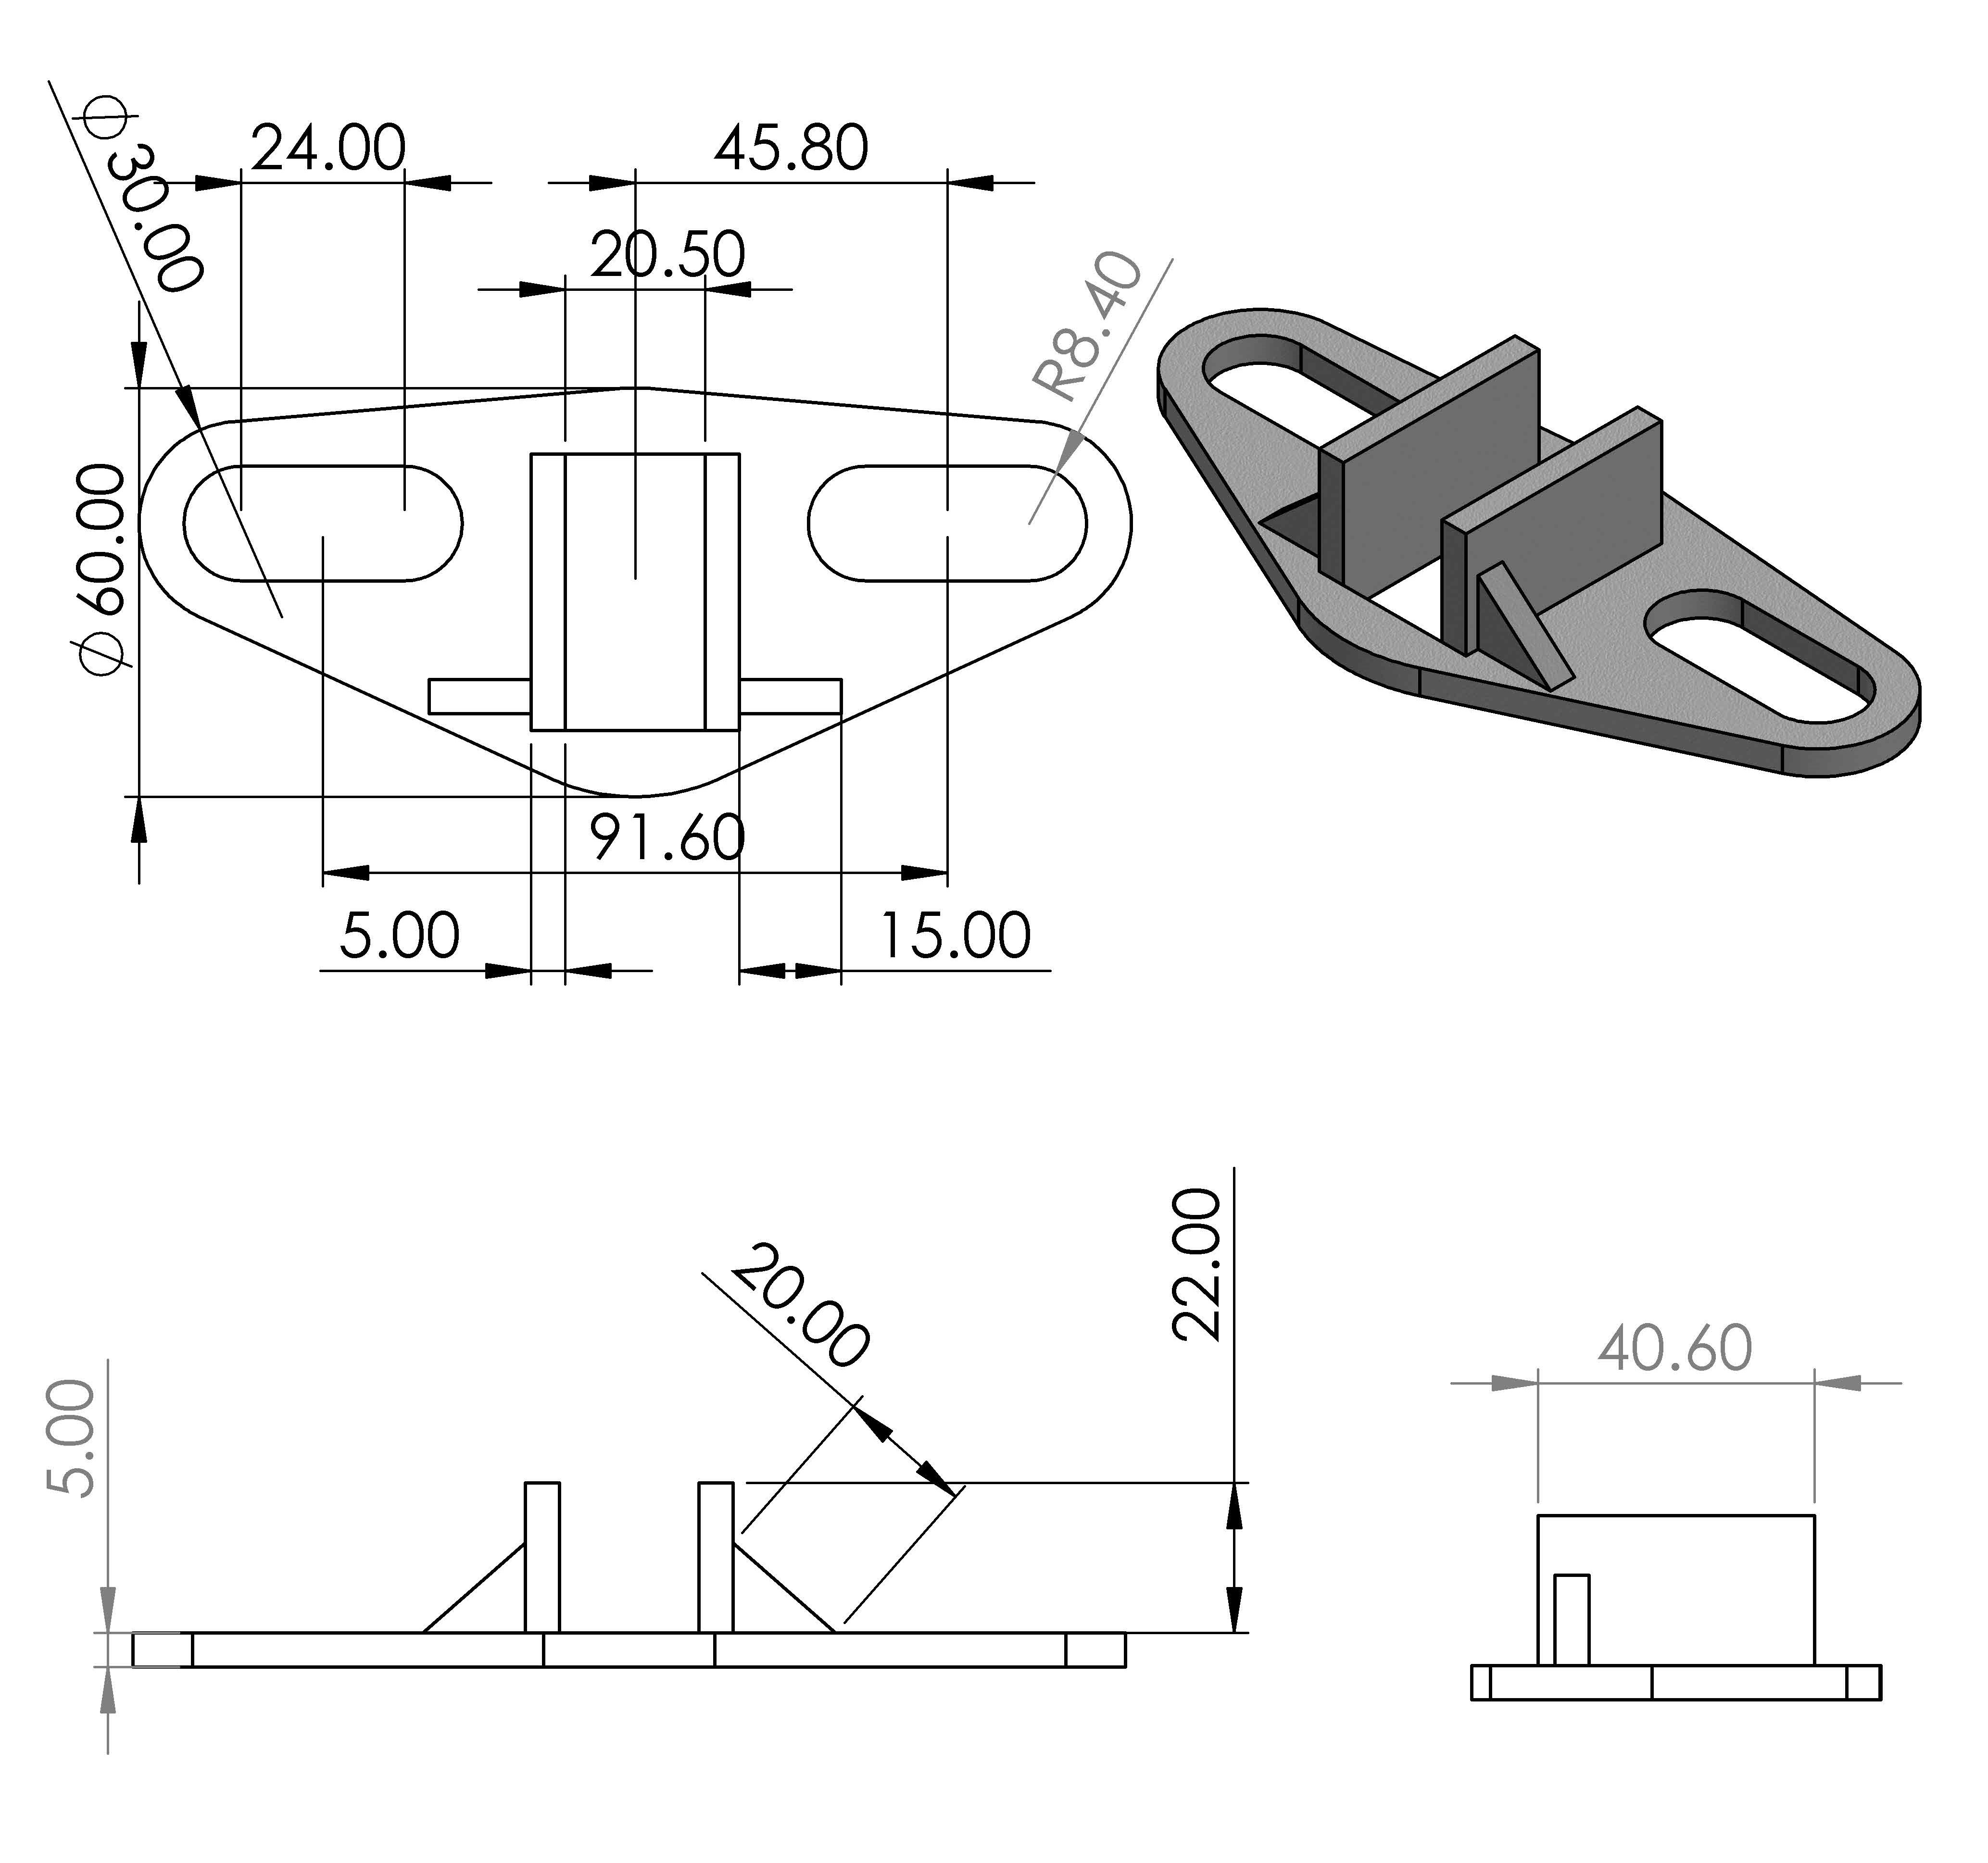
\includegraphics{Figures/ServoBracket.JPG}
\caption{Servo motor bracket}
\label{fig: Servo Holder}
\end{figure}

The fabrication was done on an Ultimaker 3D printer. The process involved the conversion of the 3D CAD model into an STL file. The file was then sliced with a 40 percent infill and 0.15 mm layer height. The choice of these parameters was based on an estimation of the amount of twisting force this part would withstand on the test rig(1Nm). The printed servo motor holder is shown in figure \ref{fig:printed_servo}. 
\begin{figure}[H]
\centering
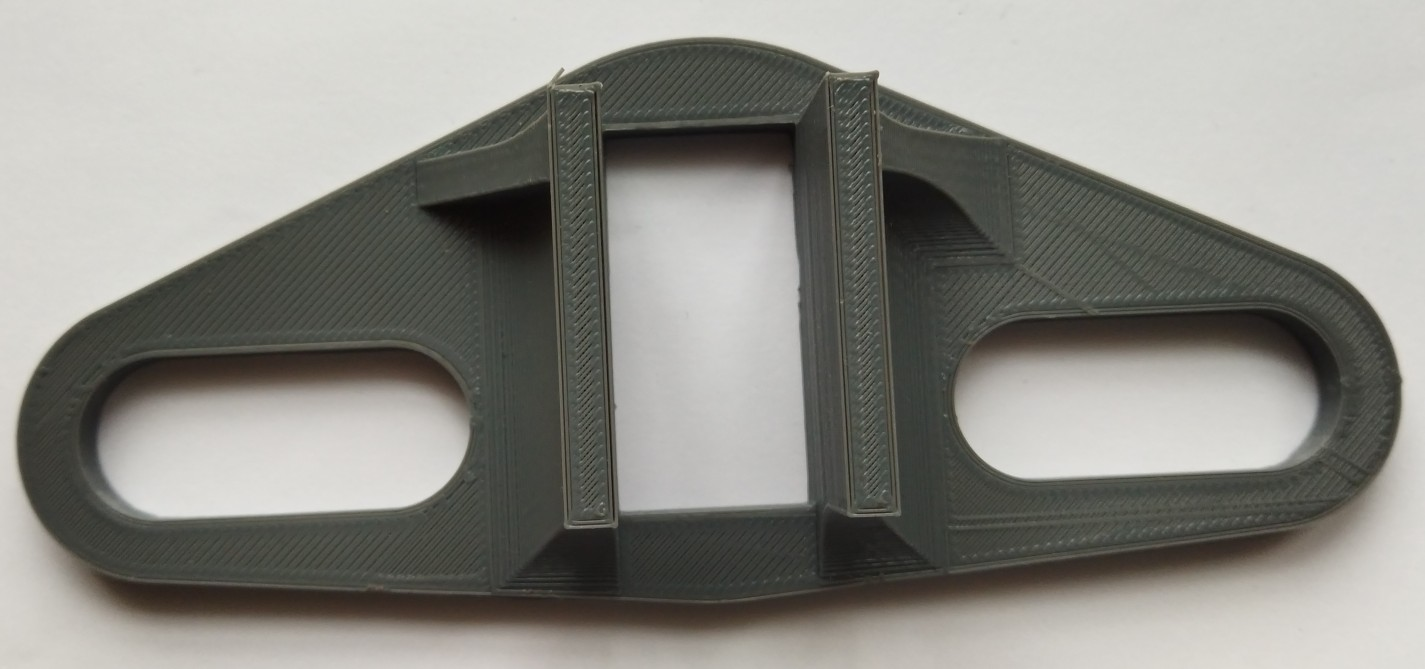
\includegraphics [width=.40\textwidth]{Figures/servoholder.jpg}
\caption{3D printed Servo Holder}
\label{fig:printed_servo}
\end{figure}  
    \item \textbf{LA-T8 holder}\\
The LA-T8 holder holds the linear actuator in position. Figure \ref{fig: LA-T8Holder} shows the design of the casing. The holder is mounted along the main discharge valve. It has to withstand the weight of the actuator and the diversion flap during operation.  The overall dimensions as indicated in figure \ref{fig: LA-T8Holder} of the LA-T8 holder were guided by the size of the actuator.
 \begin{figure}[H]
\centering
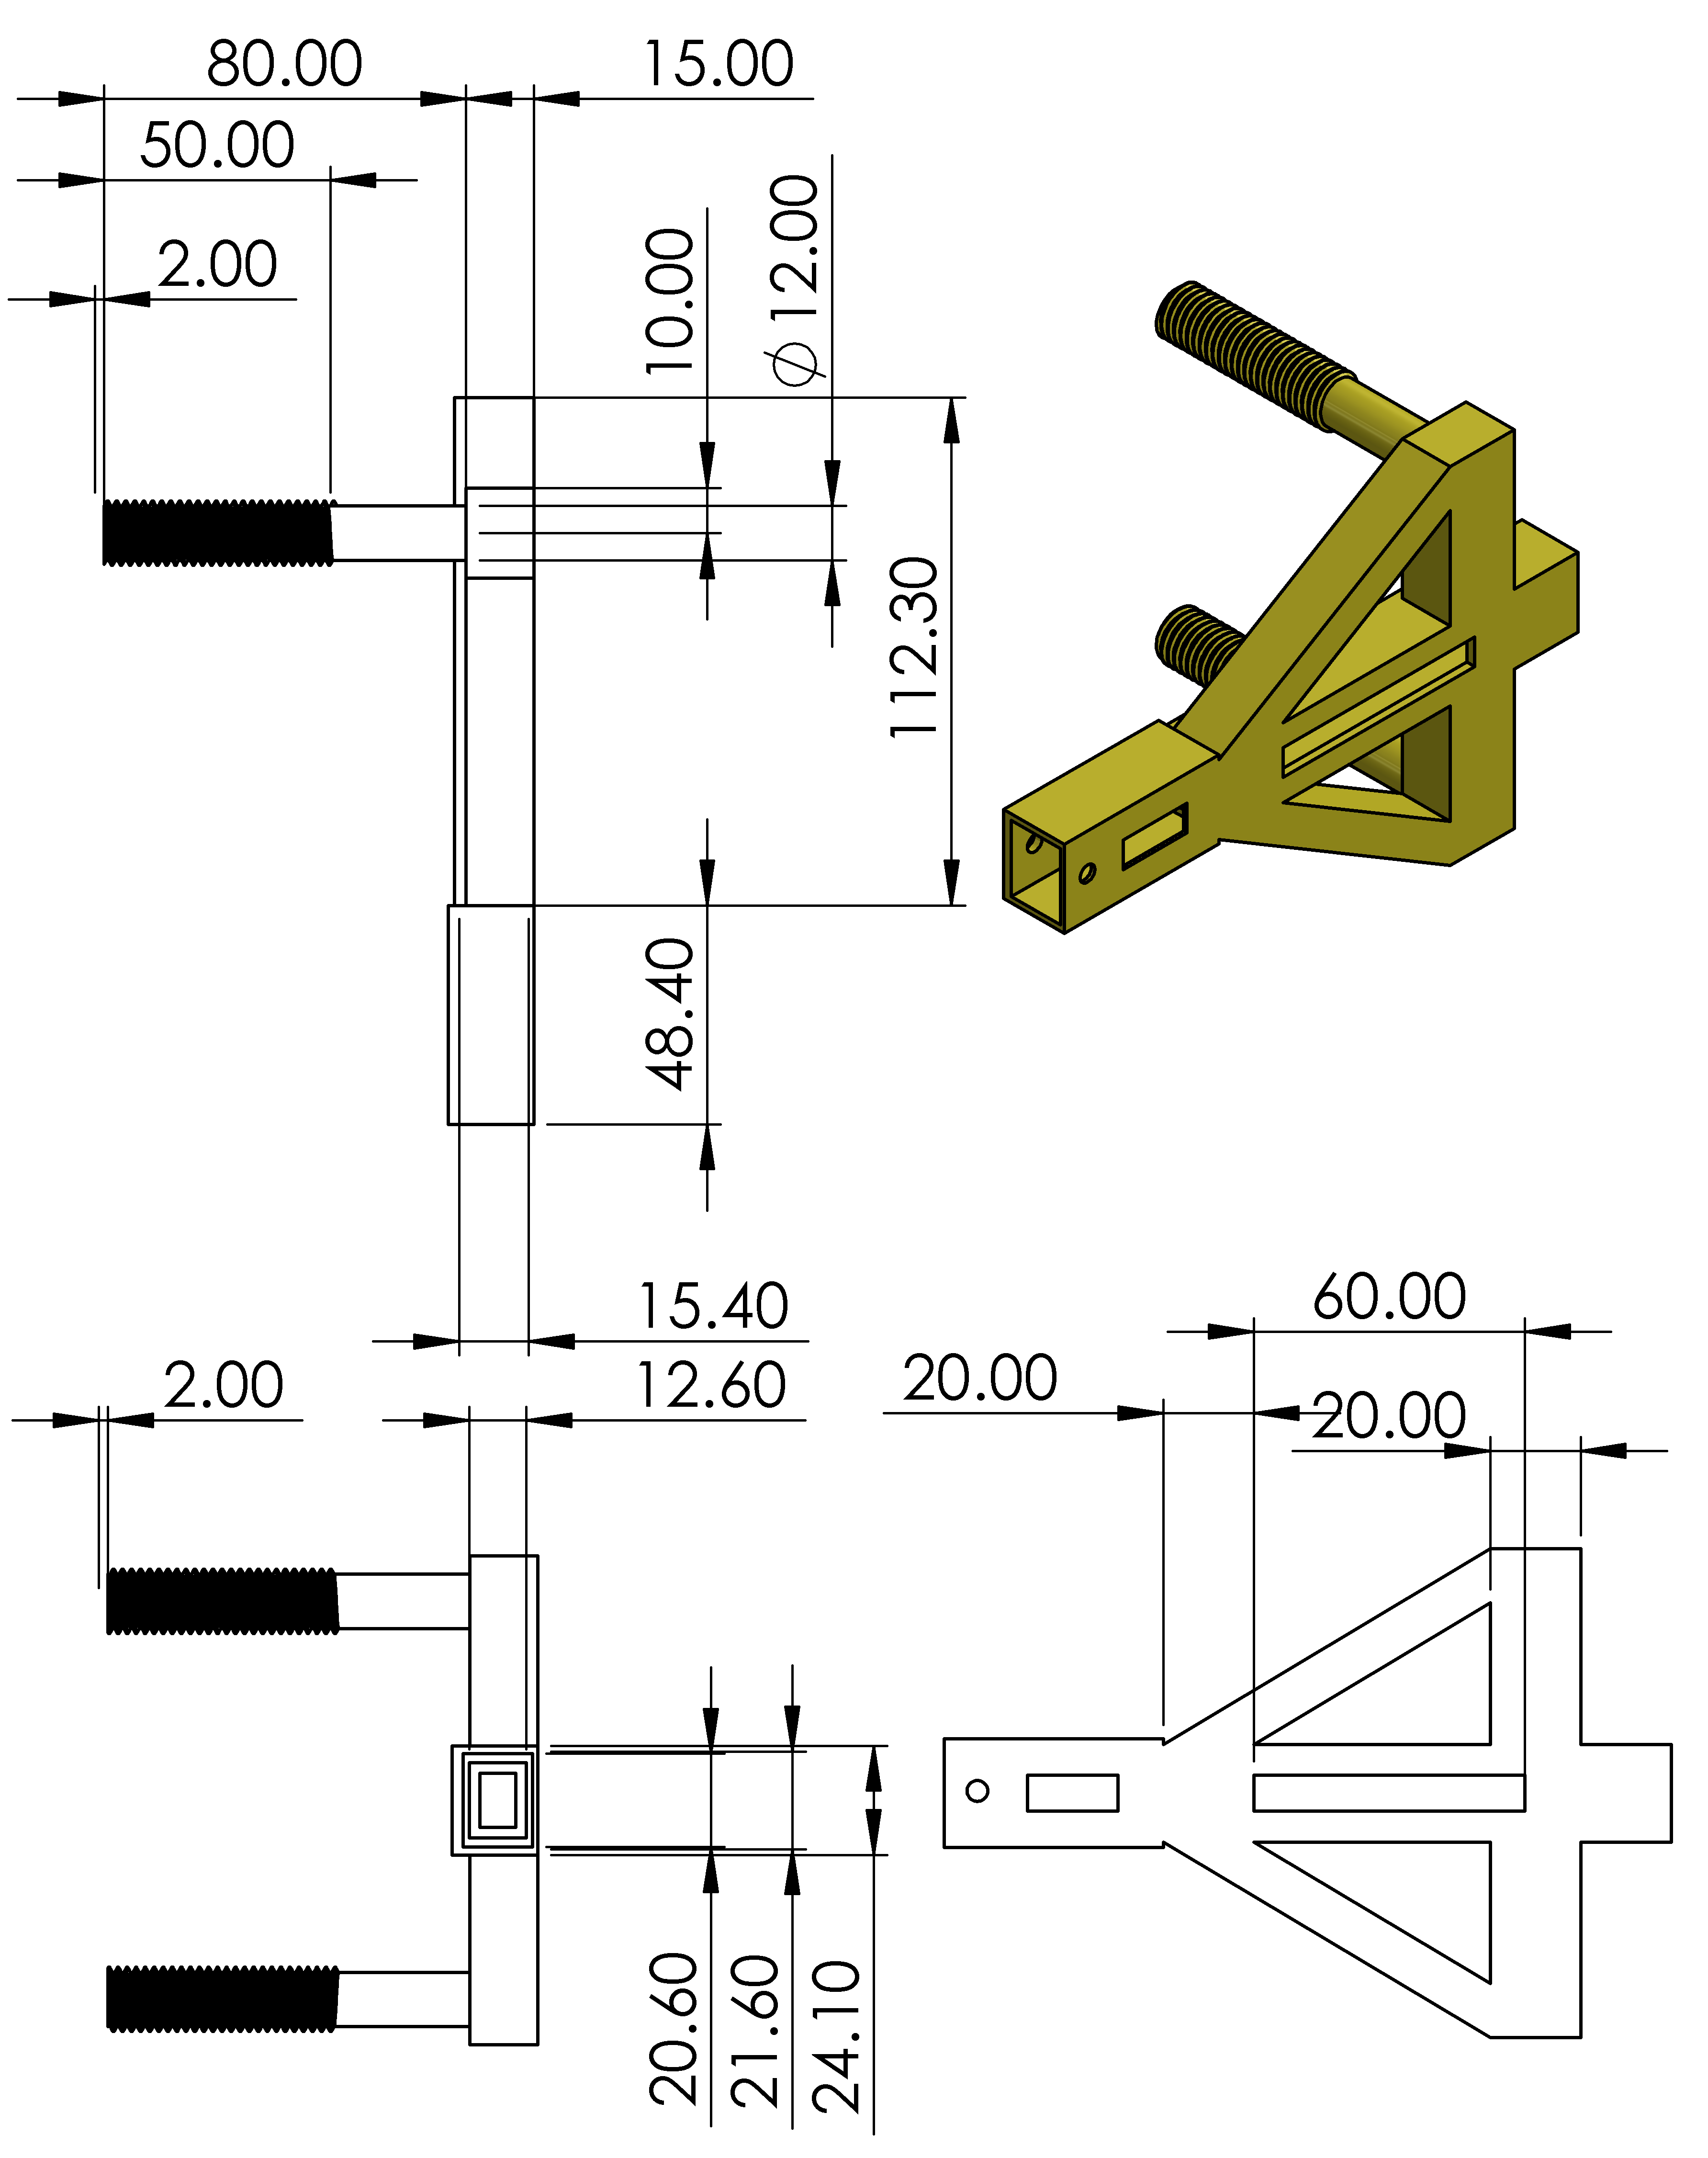
\includegraphics [width=.50\textwidth]{Figures/LA-T8Holder.PNG}
\caption{LA-T8 Holder}
\label{fig: LA-T8Holder}
\end{figure}
The width of 95mm is to enable it to be supported onto the ball valve on the machine. The holder is mounted along the main discharge pipe supporting both the diversion flap and the flap support frame. The diameter was determined from the dimensions of the straps. An allowance of 0.5mm was provided to facilitate cooling when the actuator is in operation. Additionally, the slots on the side were to reduce the overall weight of the holder. The 0.5mm holes at the tip of the holder are to bolt the actuator with the holder in place to minimize on vibrations when in operation. Besides, being operated in a water-prone environment, the LA-T8 linear actuator had to be waterproofed from any splashes of the discharge hence the above design. The final 3D printed LA-T8 holder is shown in figure \ref{fig: 3D printed LA-T8 holder} below.
\begin{figure}[H]
\centering
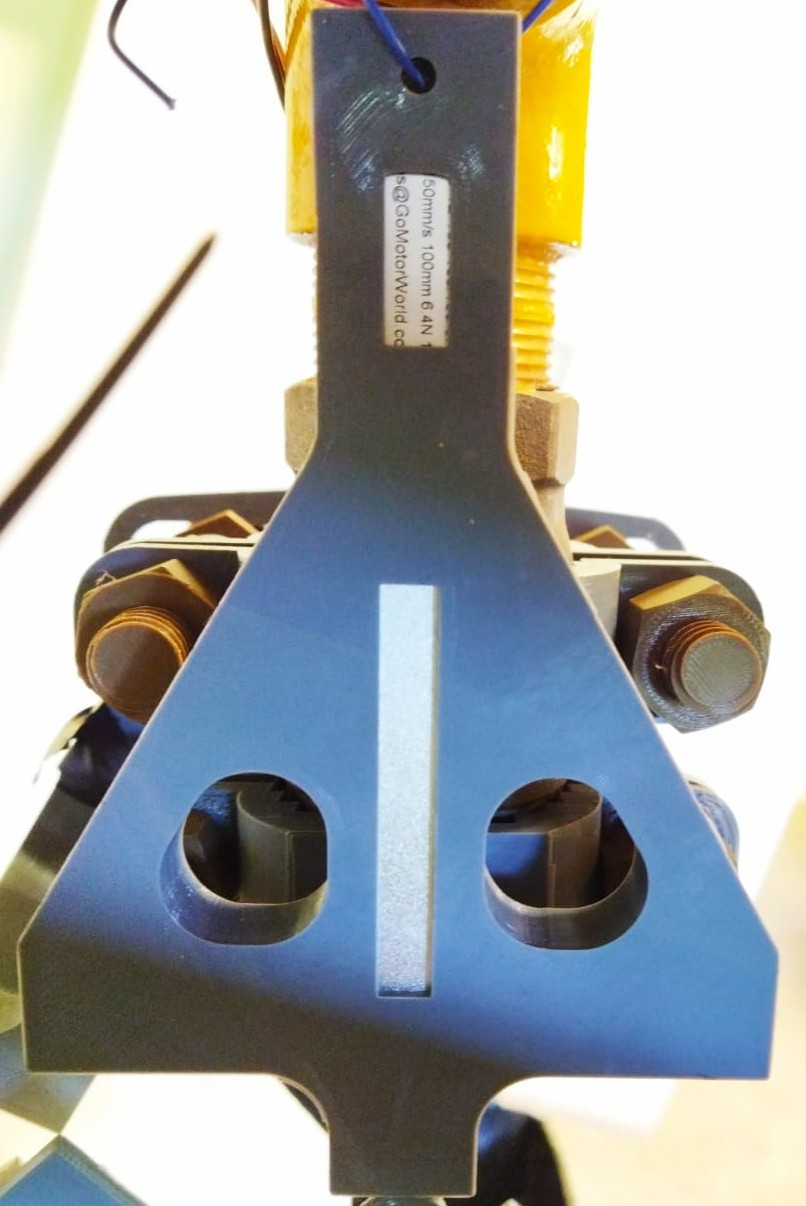
\includegraphics [width=.60\textwidth, height=.58\textheight]{Figures/laholder.jpg}
\caption{3D printed LA-T8 holder}
\label{fig: 3D printed LA-T8 holder}
\end{figure}
 \item \textbf{Straps}\\
The serrated straps and mounting rods are used to hold the servo motor and the diversion flap in position. A total of four were used for this application. Two straps were used to hold the servo motor in place while the rest were used to mount the LA-T8 holder. Figure \ref{fig: Top Strap} and \ref{fig: Bottom Strap} show the 3D CAD designs of the top and bottom straps respectively.
\begin{figure}[H]
\centering
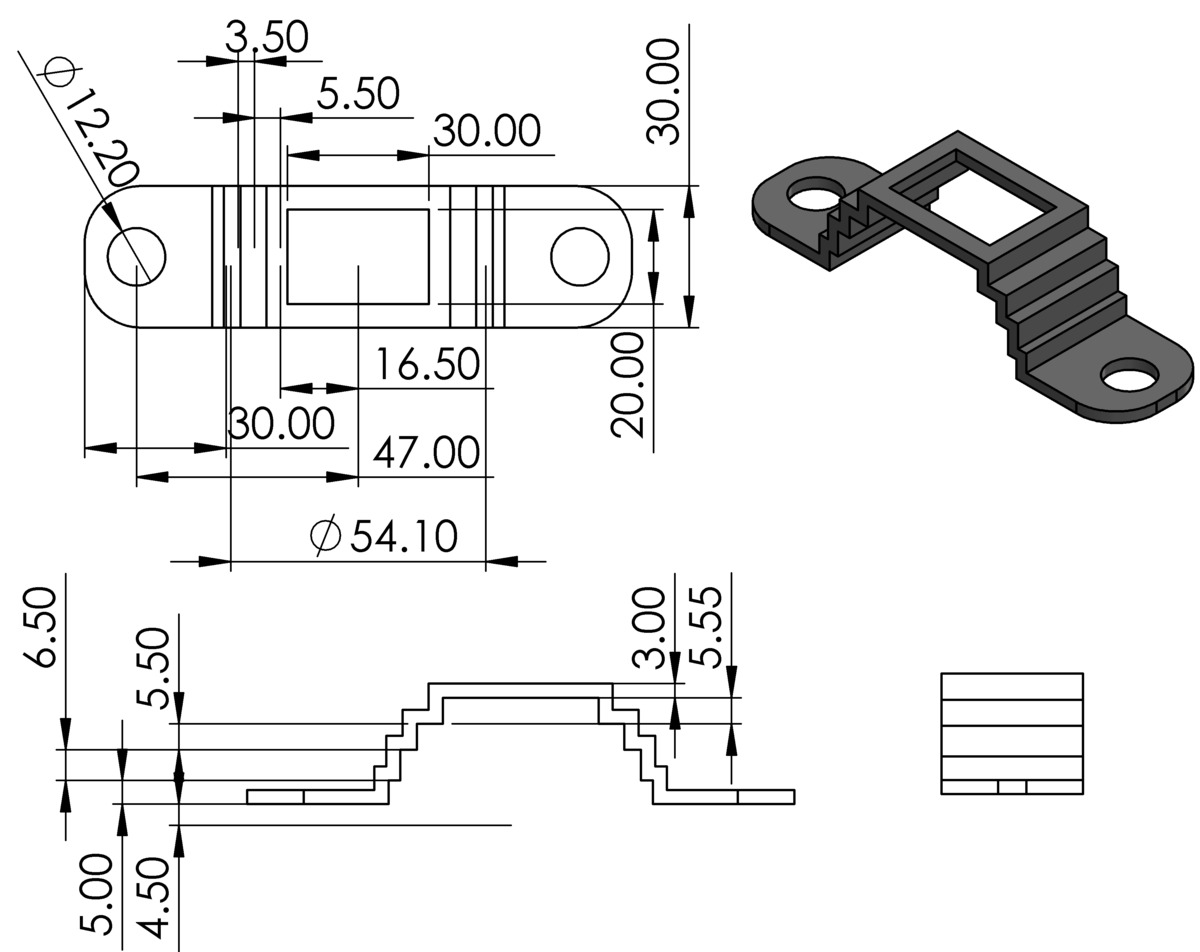
\includegraphics [width=.8\textwidth]{Figures/twoRailStrapsTop.jpg}
\caption{Top Strap}
\label{fig: Top Strap}
\end{figure}
The overall dimensions of the top strap in figure \ref{fig: Top Strap} were a total length of 114mm with an internal diameter of 54mm. The strap is mounted on the existing ball valve casing on the machine with a diameter of 50mm hence the equivalent dimensions. The extra additional 4mm in diameter was to facilitate the ease of mounting the two straps together (top and bottom) to ensure that they firmly fit. The square pocket on the top strap was to allow for the mounting of the valve interface. The 30mm by 30mm dimensions were dependent on the protruding dimensions of the existing ball valve casing. The serrations on the straps were to provide more grip while at the same time supporting more load. 
\begin{figure}[H]
\centering
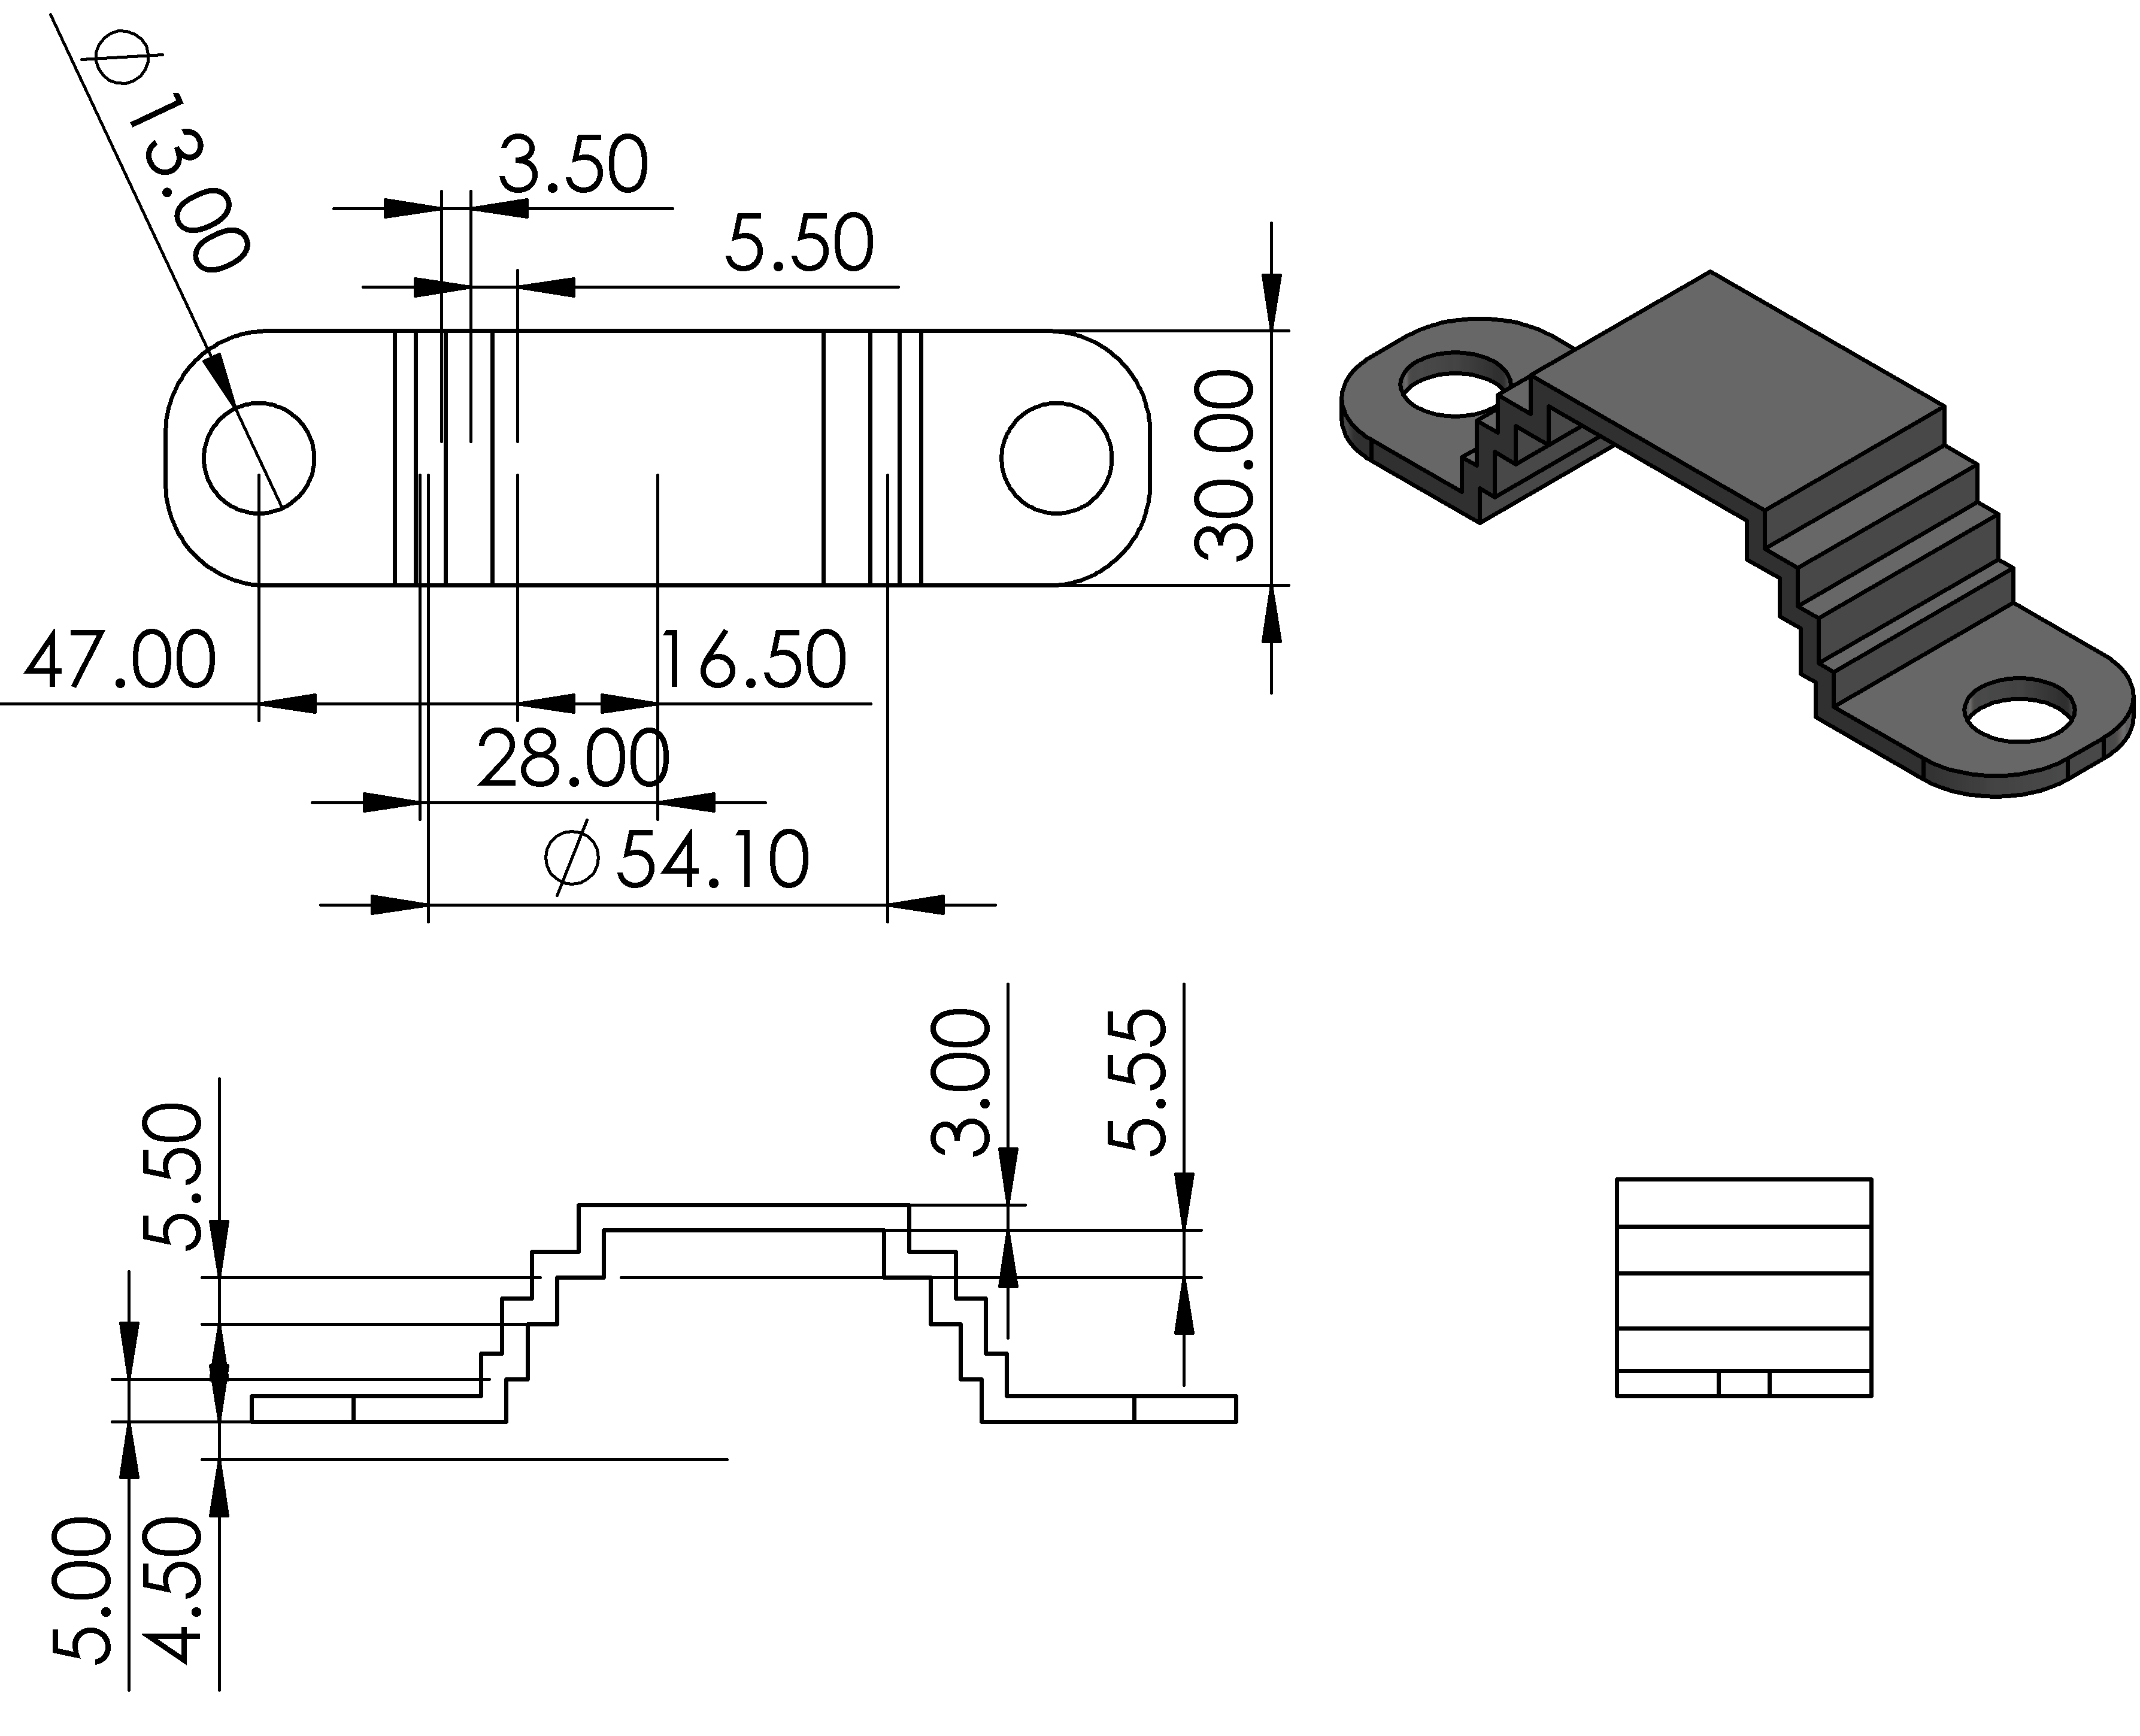
\includegraphics [width=.8\textwidth]{Figures/twoRailStrapsBottom.PNG}
\caption{Bottom Strap}
\label{fig: Bottom Strap}
\end{figure}
All the straps were 3D printed using the Ultimaker 3D printer. The above 3D CAD models were converted into STL files and sliced with the same settings as the servo motor bracket. Figure \ref{fig: 3D printed top and bottom straps} below shows the printed parts.
\begin{figure}[H]
    \centering
    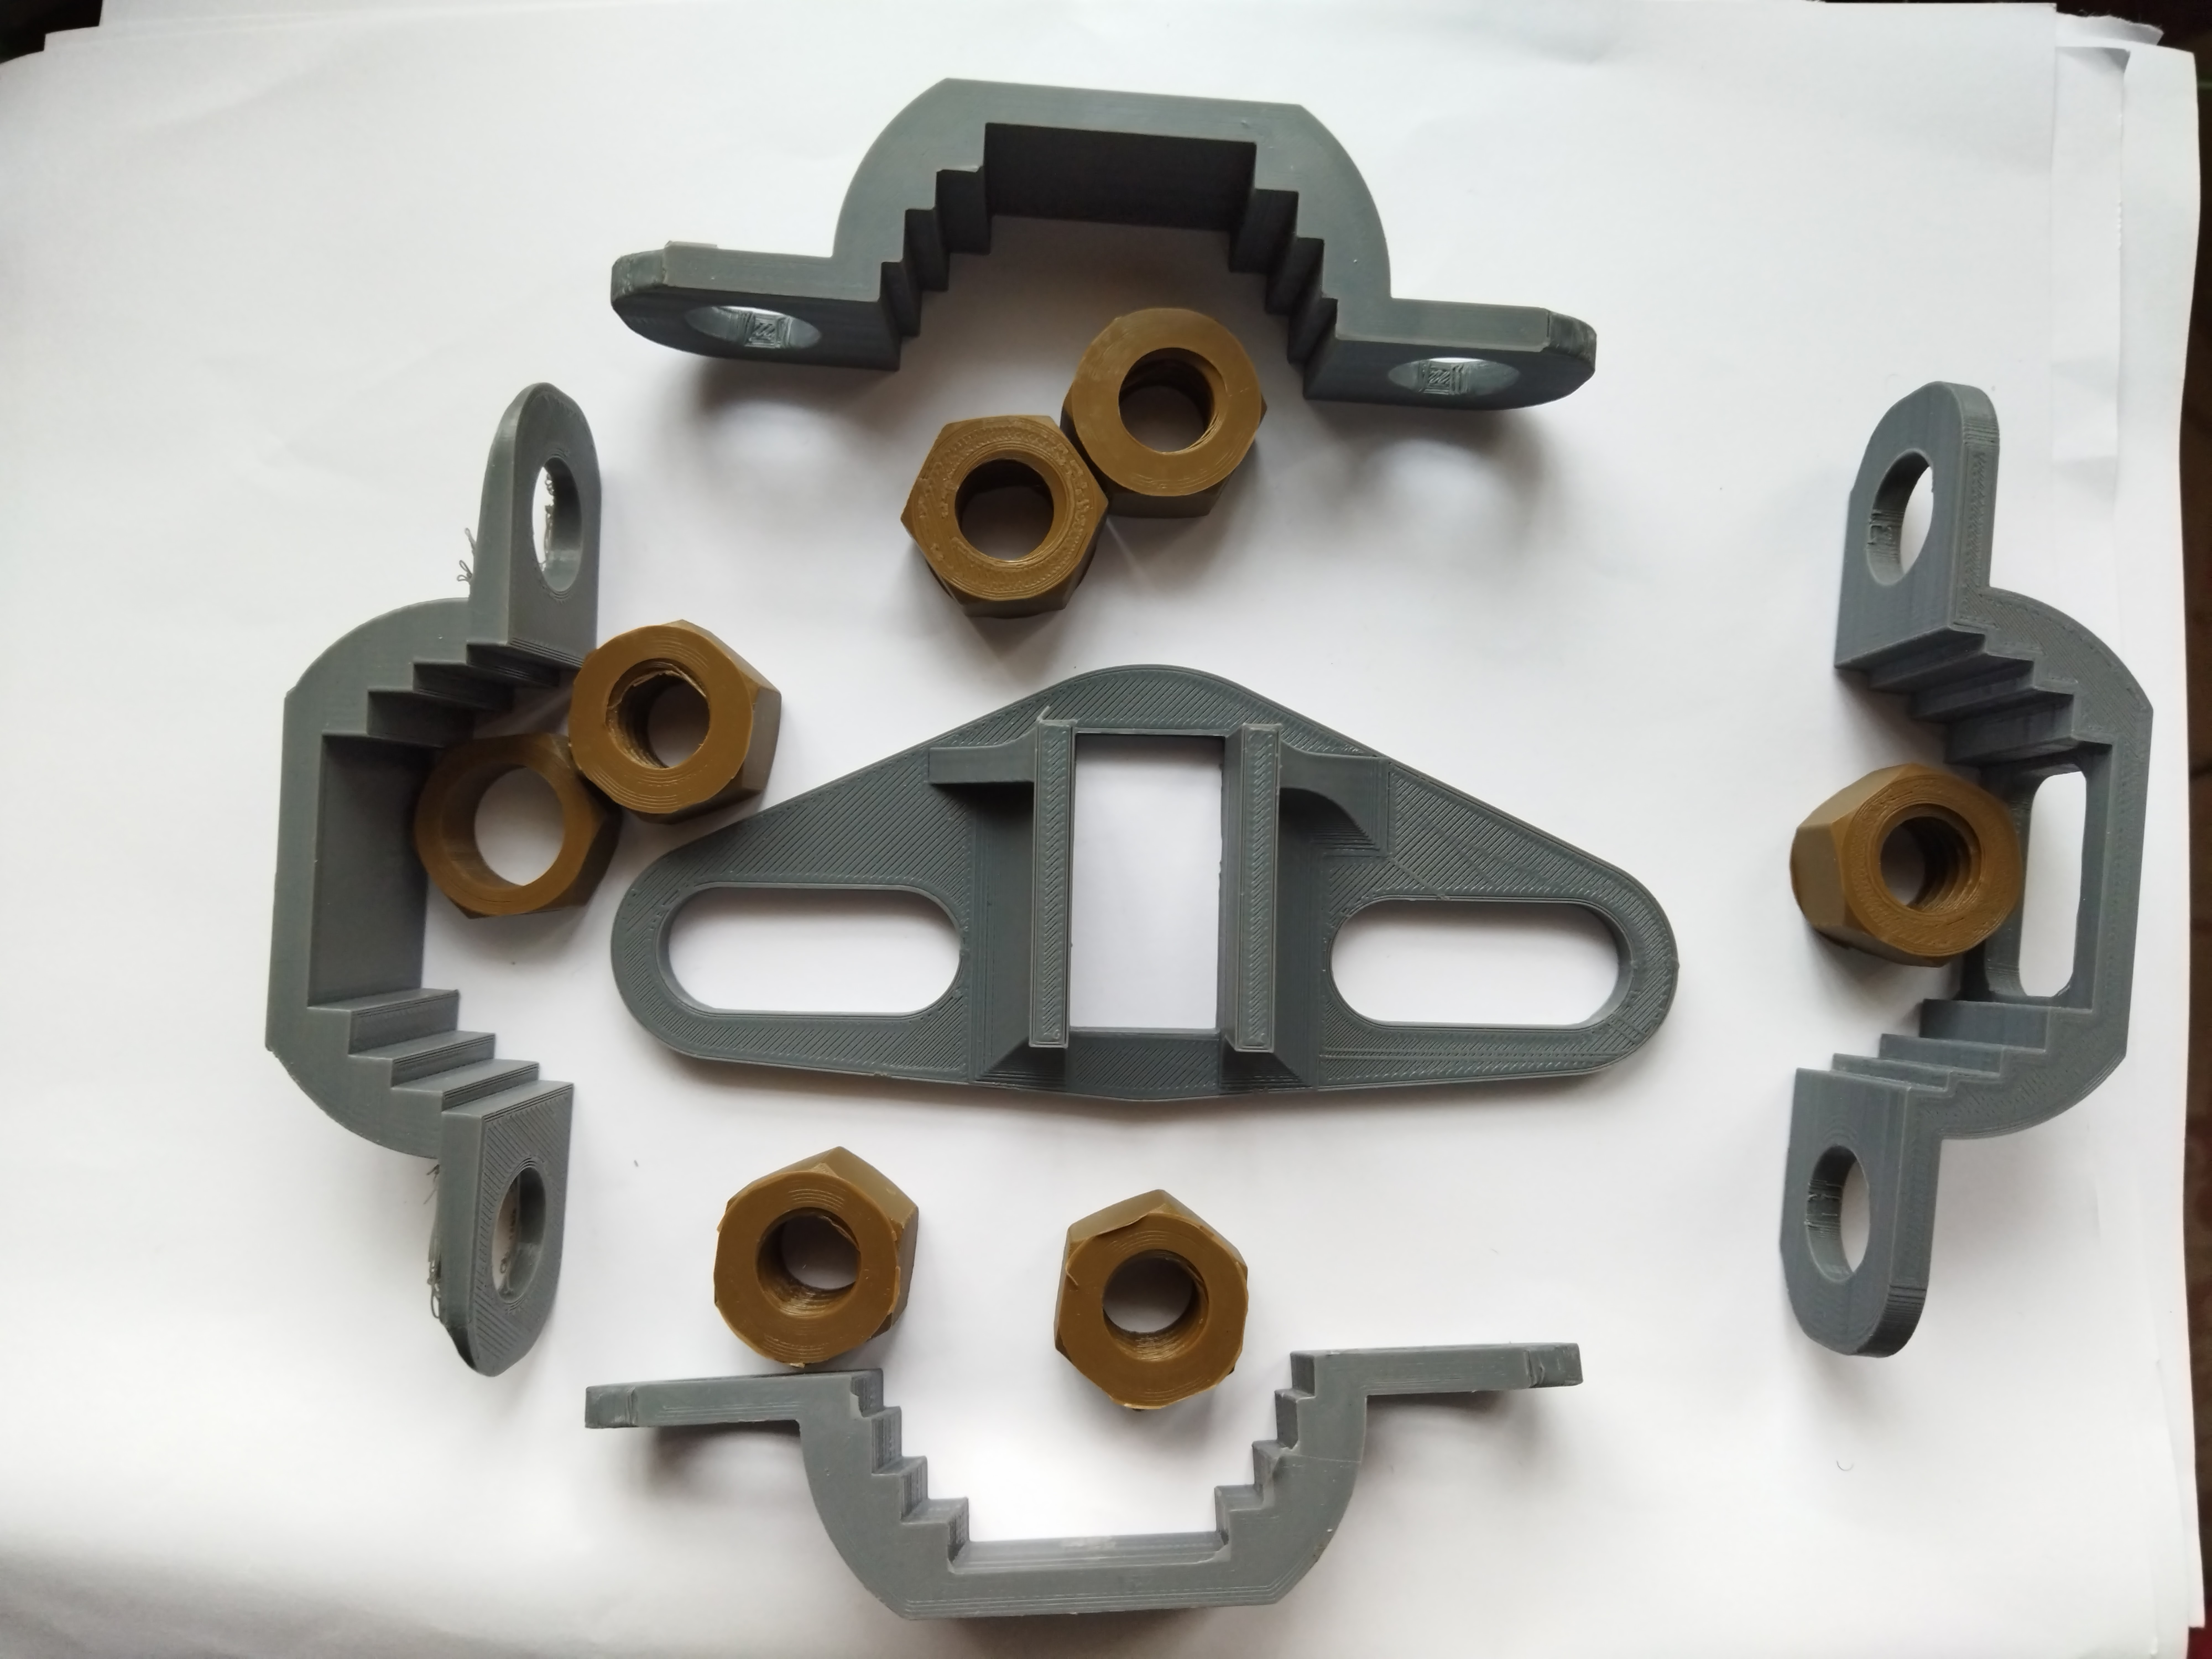
\includegraphics[width=0.8\textwidth]{Figures/IMG_20220930_073222.jpg}
    \caption{3D printed top and bottom straps}
    \label{fig: 3D printed top and bottom straps}
\end{figure}
\item \textbf{Valve interface}\\
The interface is used to connect the motor rotor to the ball valve to facilitate the actuation of the valve. Figure \ref{fig: Interface} below shows the interface design. It is fixed onto the motor using a nut while the other end is coupled to the motor shaft.
\begin{figure}[H]
\centering
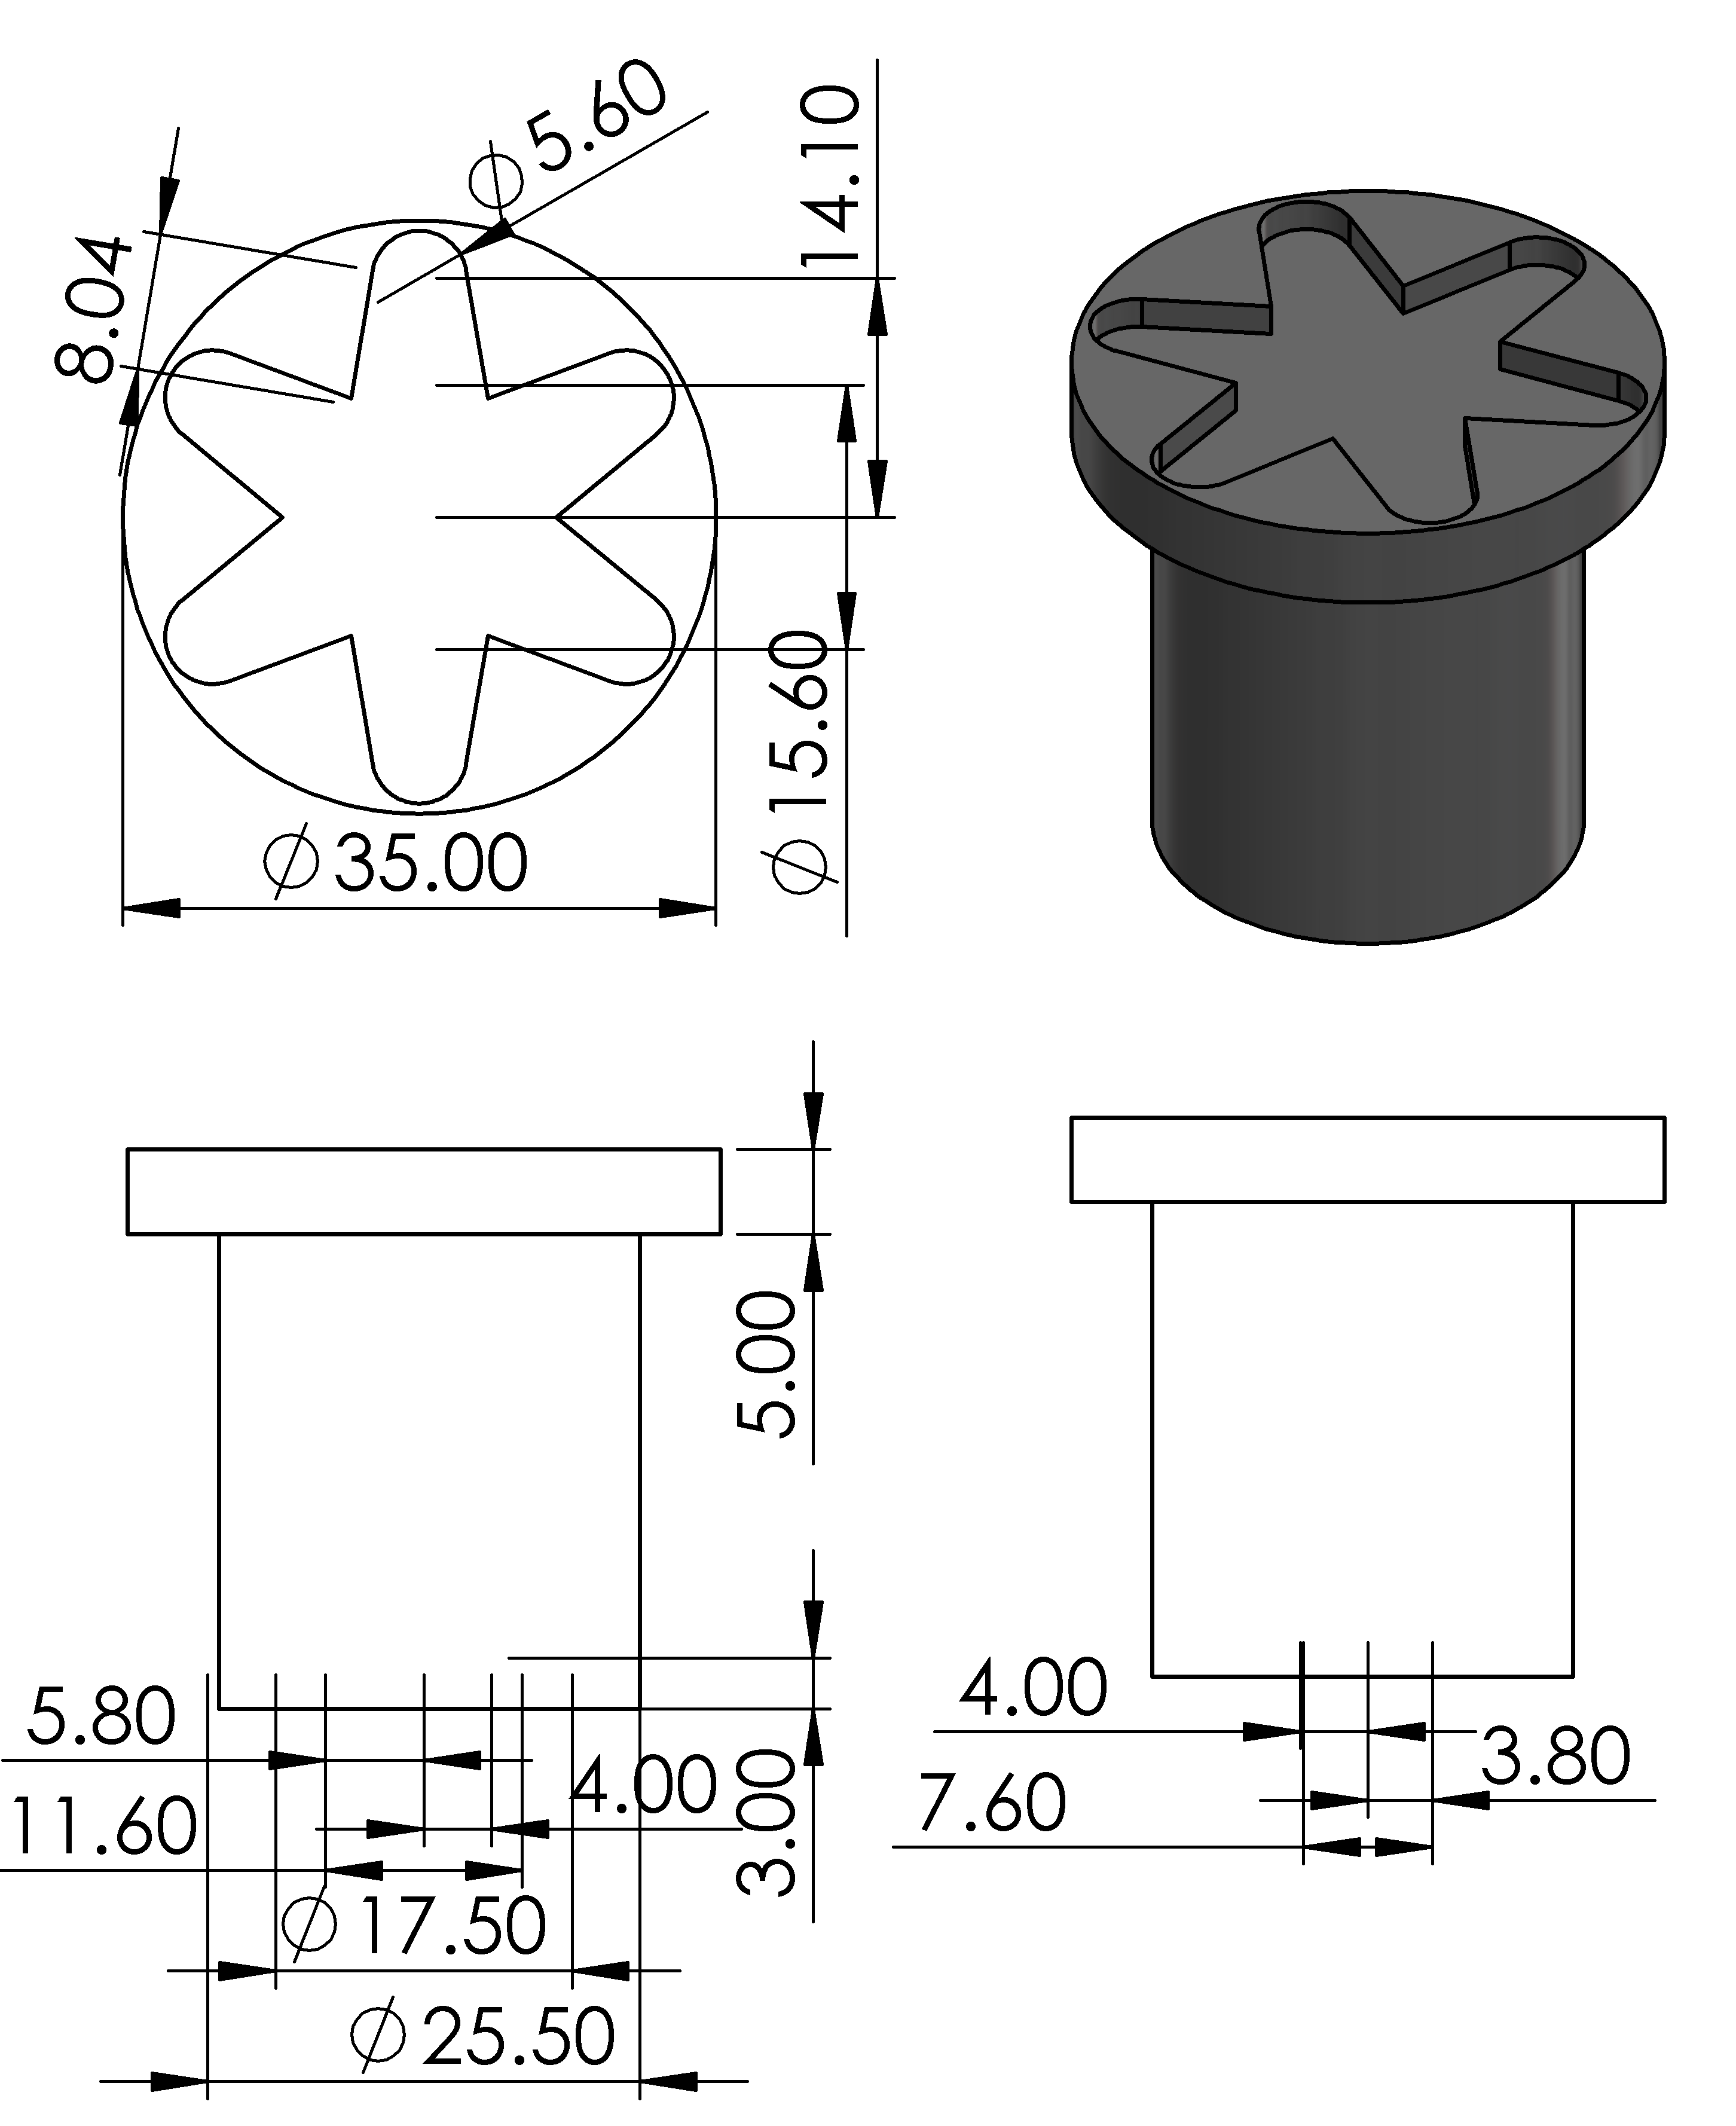
\includegraphics [width=.8\textwidth, height=.6\textheight]{Figures/interface.PNG}
\caption{Interface}
\label{fig: Interface}
\end{figure}
The dimensions of the interface such as the width of its base were measured directly and transferred from the existing ball valve. The overall height was dependent on the mounting rods hence the equivalent dimensions. 
\item \textbf{Diversion Flap}\\
To divert the discharge, a channel-like flap is used. The design of the flap is shown in figure \ref{fig: Diversion Flap}. The design was such that it can tap the whole stream from the $1\frac{3}{4} inch$ main discharge pipe on the hydraulics test rig. 
\begin{figure}[H]
\centering
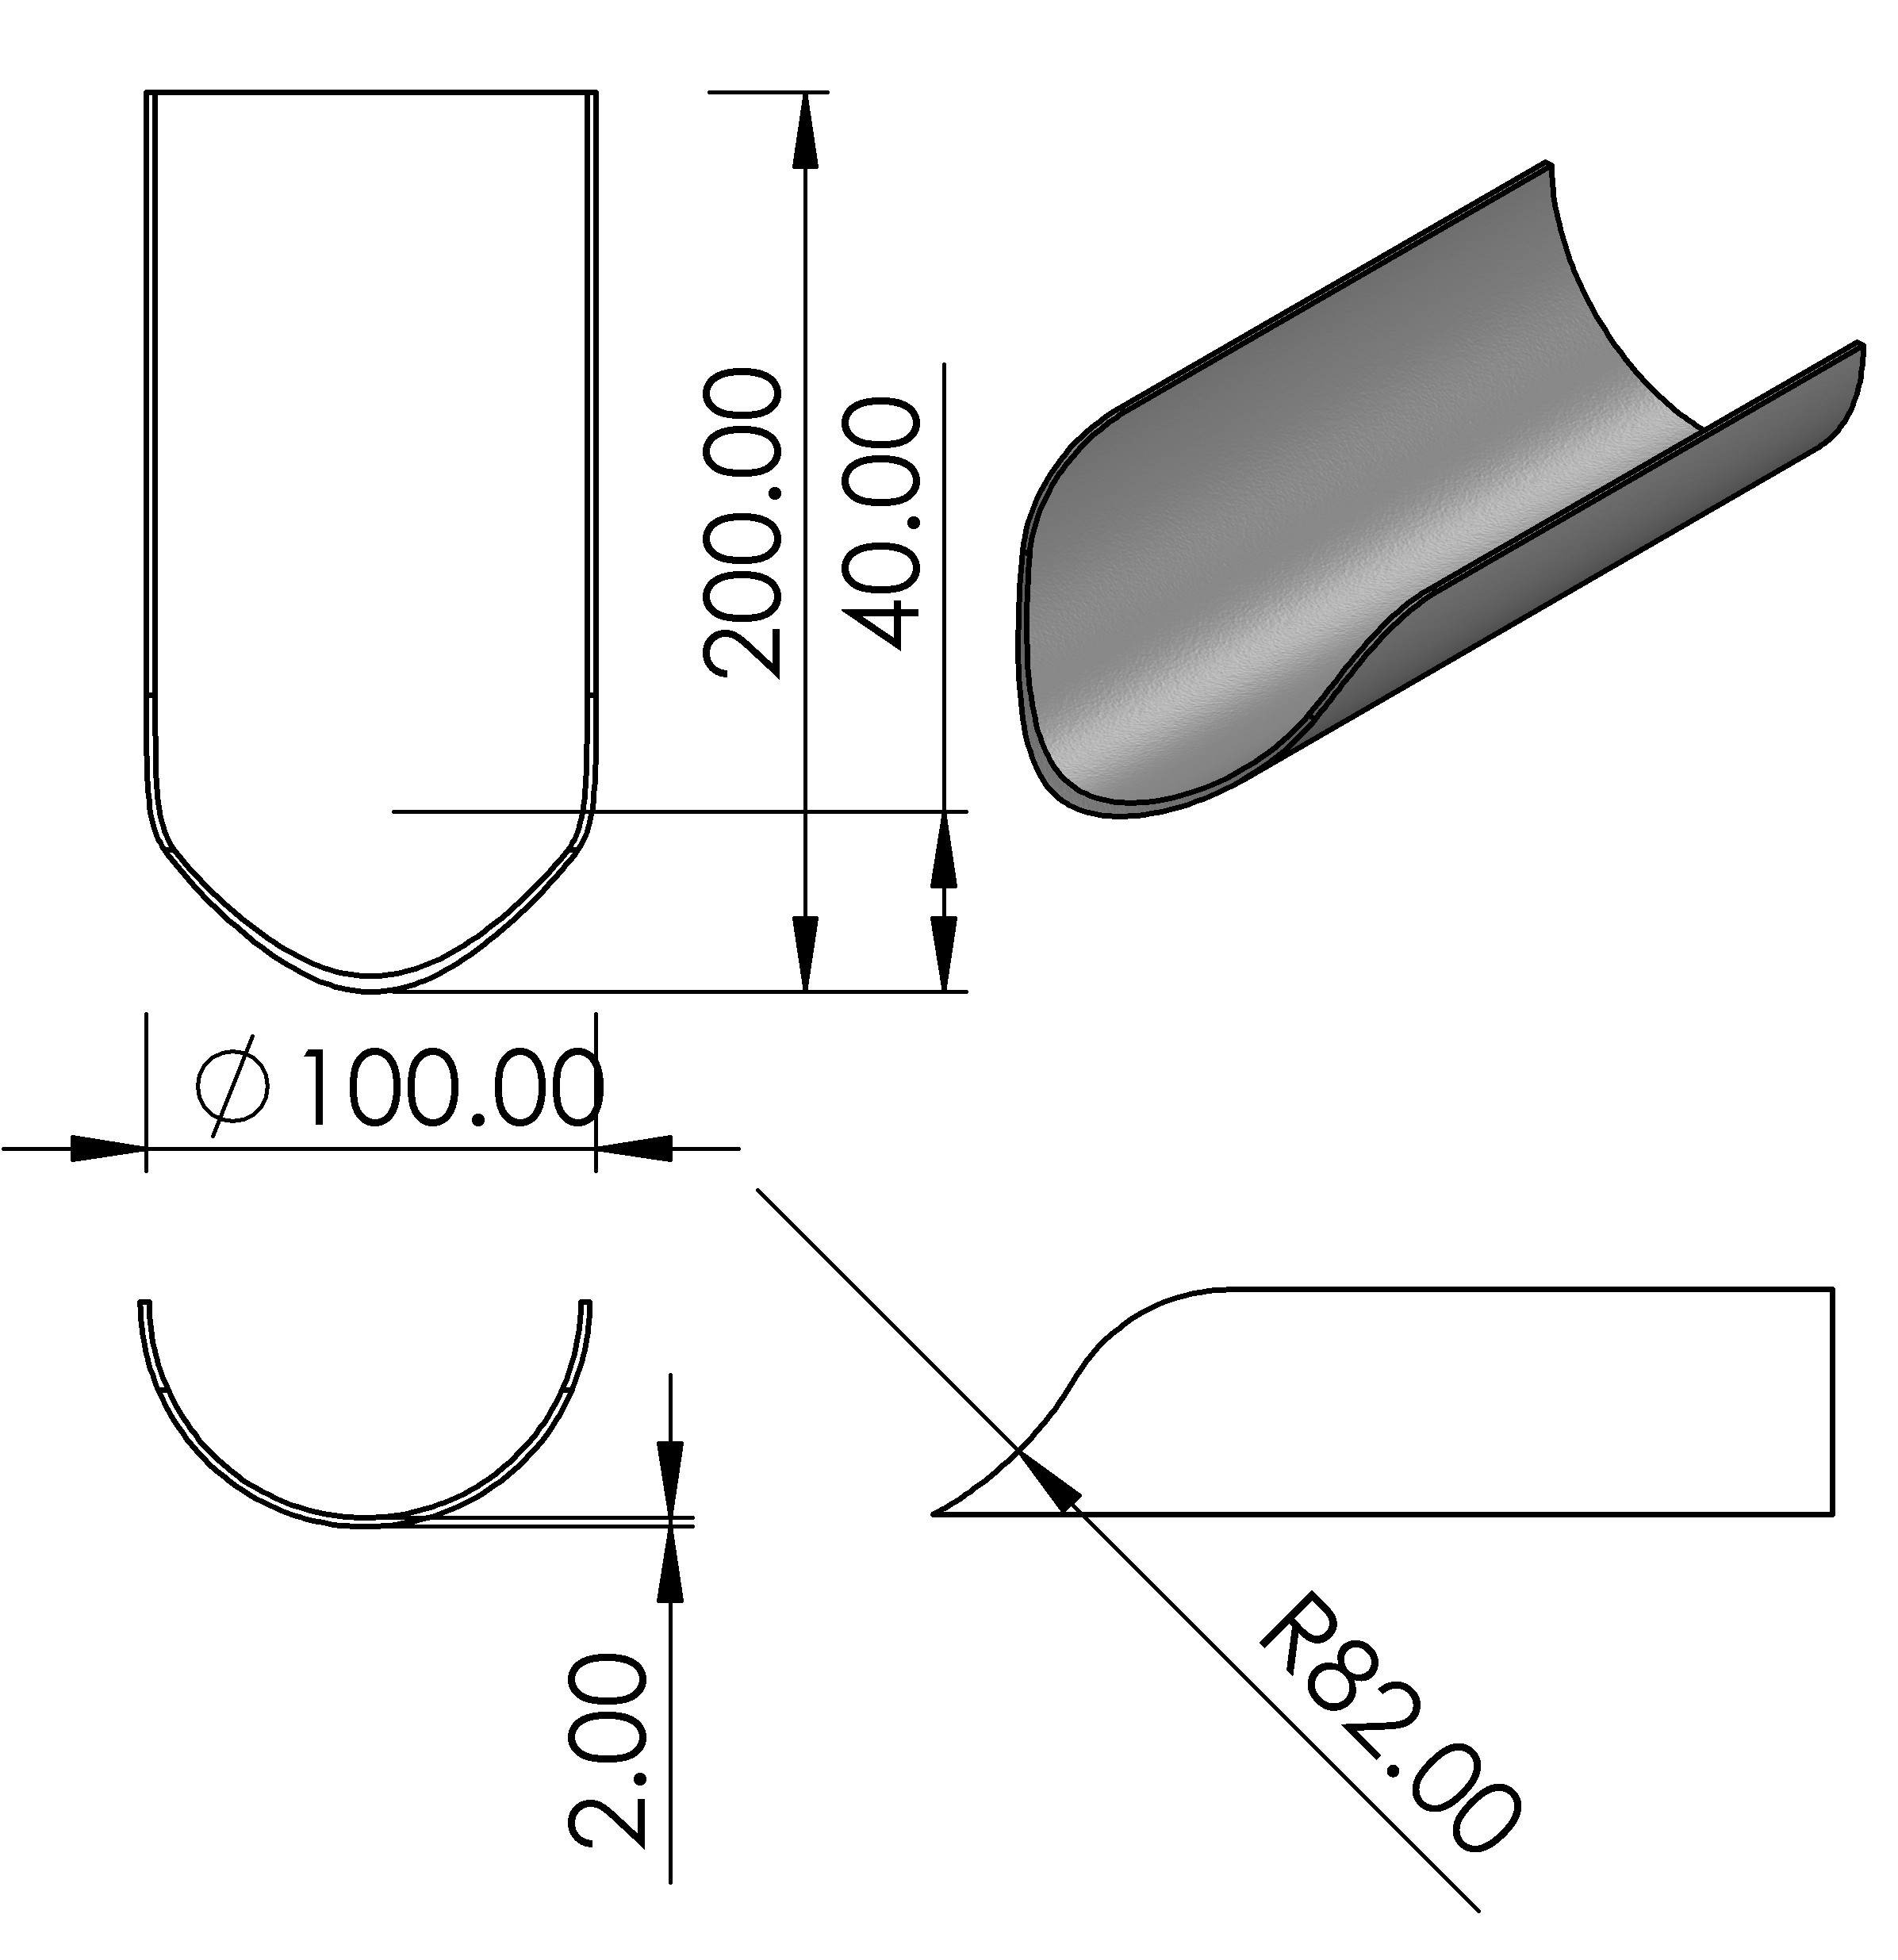
\includegraphics [width=.8\textwidth]{Figures/flap2.PNG}
\caption{Diversion Flap}
\label{fig: Diversion Flap}
\end{figure}
The flap was cut from a polyvinyl chloride (PVC) pipe as per the design dimensions. The 200mm length was determined by the length of the gap between the discharge pipe and the collection tank. It was necessary to ensure that there was free movement of the flap for proper diversion and no strain on the linear actuator. The dimensions of the selected PVC more so the width were guided by the diameter of the discharge pipe.
\item \textbf{Mounting Rods}\\
Two mounting rods are used to support the mounted servo motor assembly on the ball valve casing. The design of the rod is as shown in figure \ref{fig: Mounting Rod}.
\begin{figure}[H]
\centering
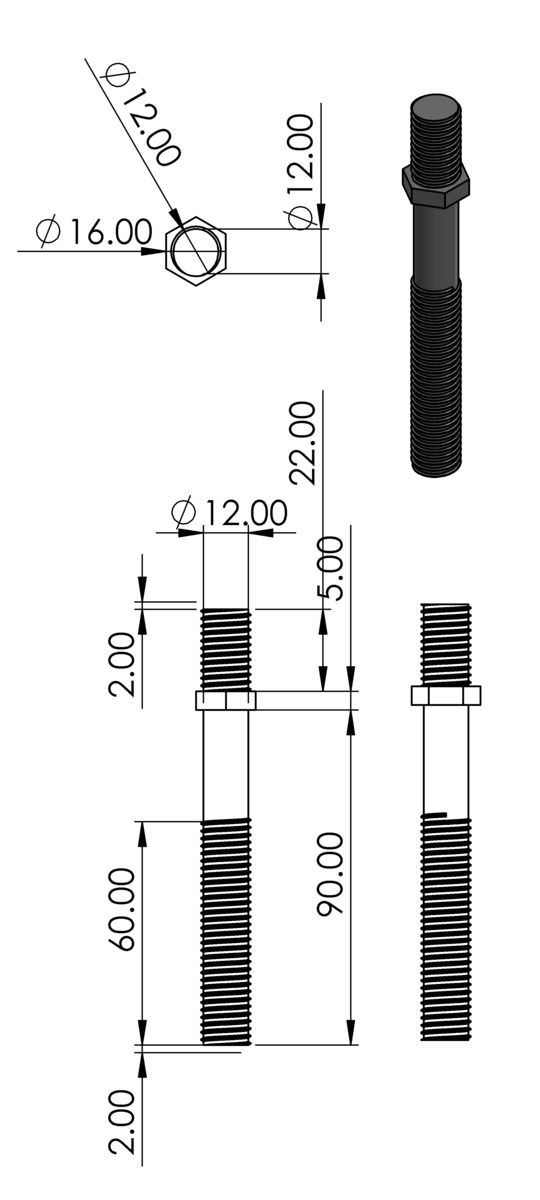
\includegraphics [width=.5\textwidth]{Figures/ServoMotorMountRods.jpg}
\caption{Mounting Rod}
\label{fig: Mounting Rod}
\end{figure}
The choice to 3D print the mounting rods was the fact that the design allows for the fasteners on both sides; at one end to fasten the servo motor assembly after alignment and on the other end to fasten the whole flow control unit on the main discharge flow pipe with the help of serrated straps. The protrusion on the surface eliminates the need for another fastener which would add to the overall complexity of the system. Figure \ref{fig: 3D printed Mounting Rod} shows the 3D printed mounting rods. 
\begin{figure}[H]
\centering
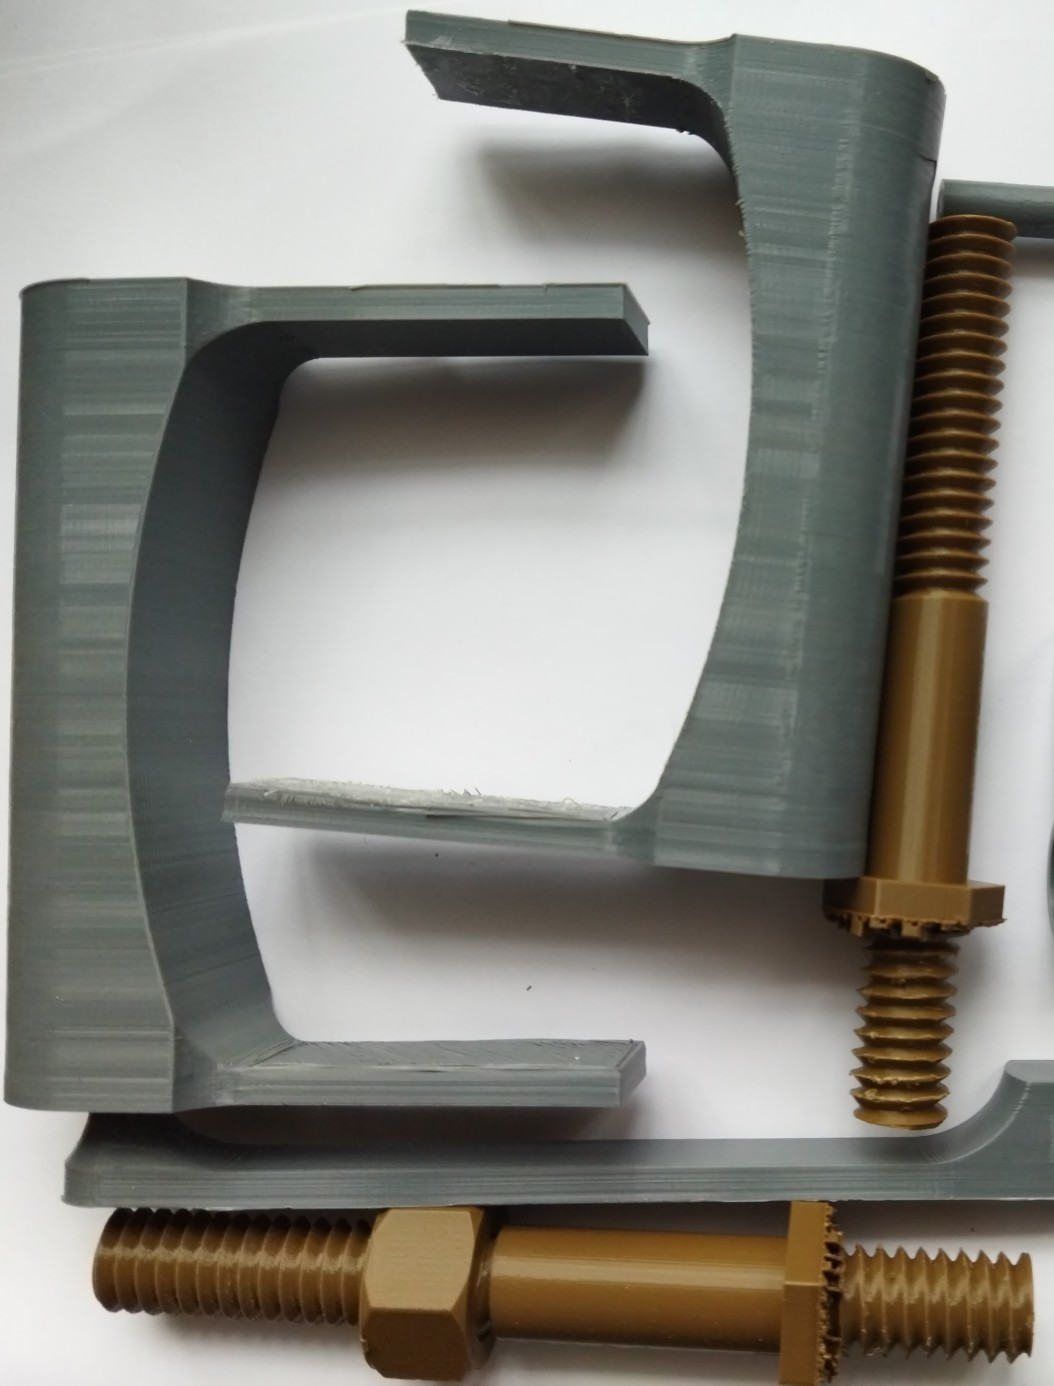
\includegraphics [height=.6\textheight] {Figures/de.jpg}
\caption{Mounting Rod}
\label{fig: 3D printed Mounting Rod}
\end{figure}
\end{enumerate}

\subsubsection{Material selection}
All the components from the servo motor holder, the LA-T8 linear actuator holder, a diversion flap, links, mounting straps, an interface, and mounting rods were all made from Polylactic acid (PLA). PLA was used due to its ease of use and minimal warping issues. The diversion flap is made from polyvinyl chloride (PVC). Furthermore, the use of PLA and PVC served two main functions. The first was to eliminate the rusting of components that would have arisen with the use of metallic components. Secondly, was to cut down on the overall cost as it would not require preventive processes to prevent rusting.
\subsubsection{Design Modifications}
\begin{itemize}
    \item \textbf{Link}\\
The link that serves to connect the linear actuator to the diversion flap was changed from that in figure \ref{fig: Link 1} to that in figure \ref{fig: Link 2} with the main modification being increasing the overall thickness of the link.
\begin{figure}[H]
\centering
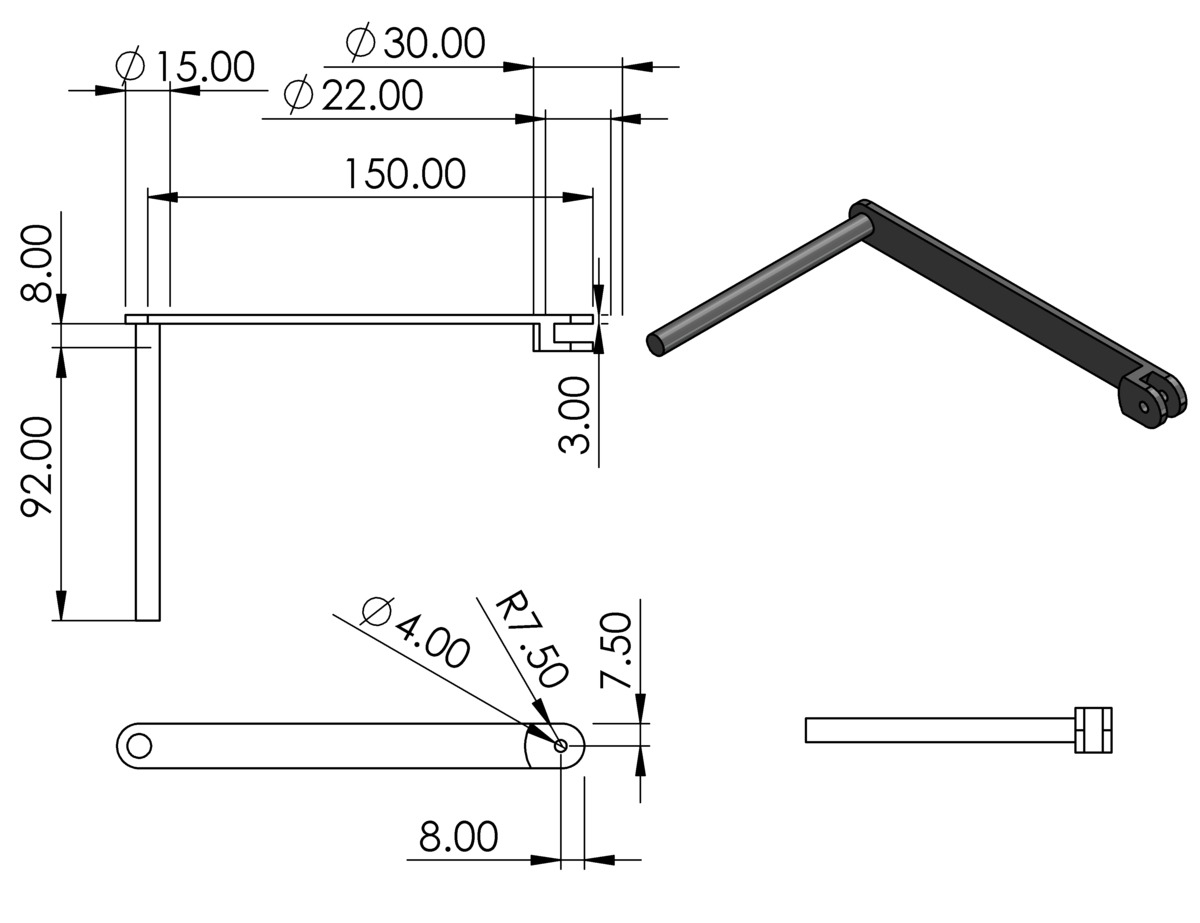
\includegraphics [width=.8\textwidth] {Figures/RockerLink.jpg}
\caption{Link1}
\label{fig: Link 1}
\end{figure}
The thickness of the link was increased from 3mm to 5mm. This was because the initial link was warping under loading conditions when the flow was at its maximum pressure.        
\begin{figure}[H]
\centering
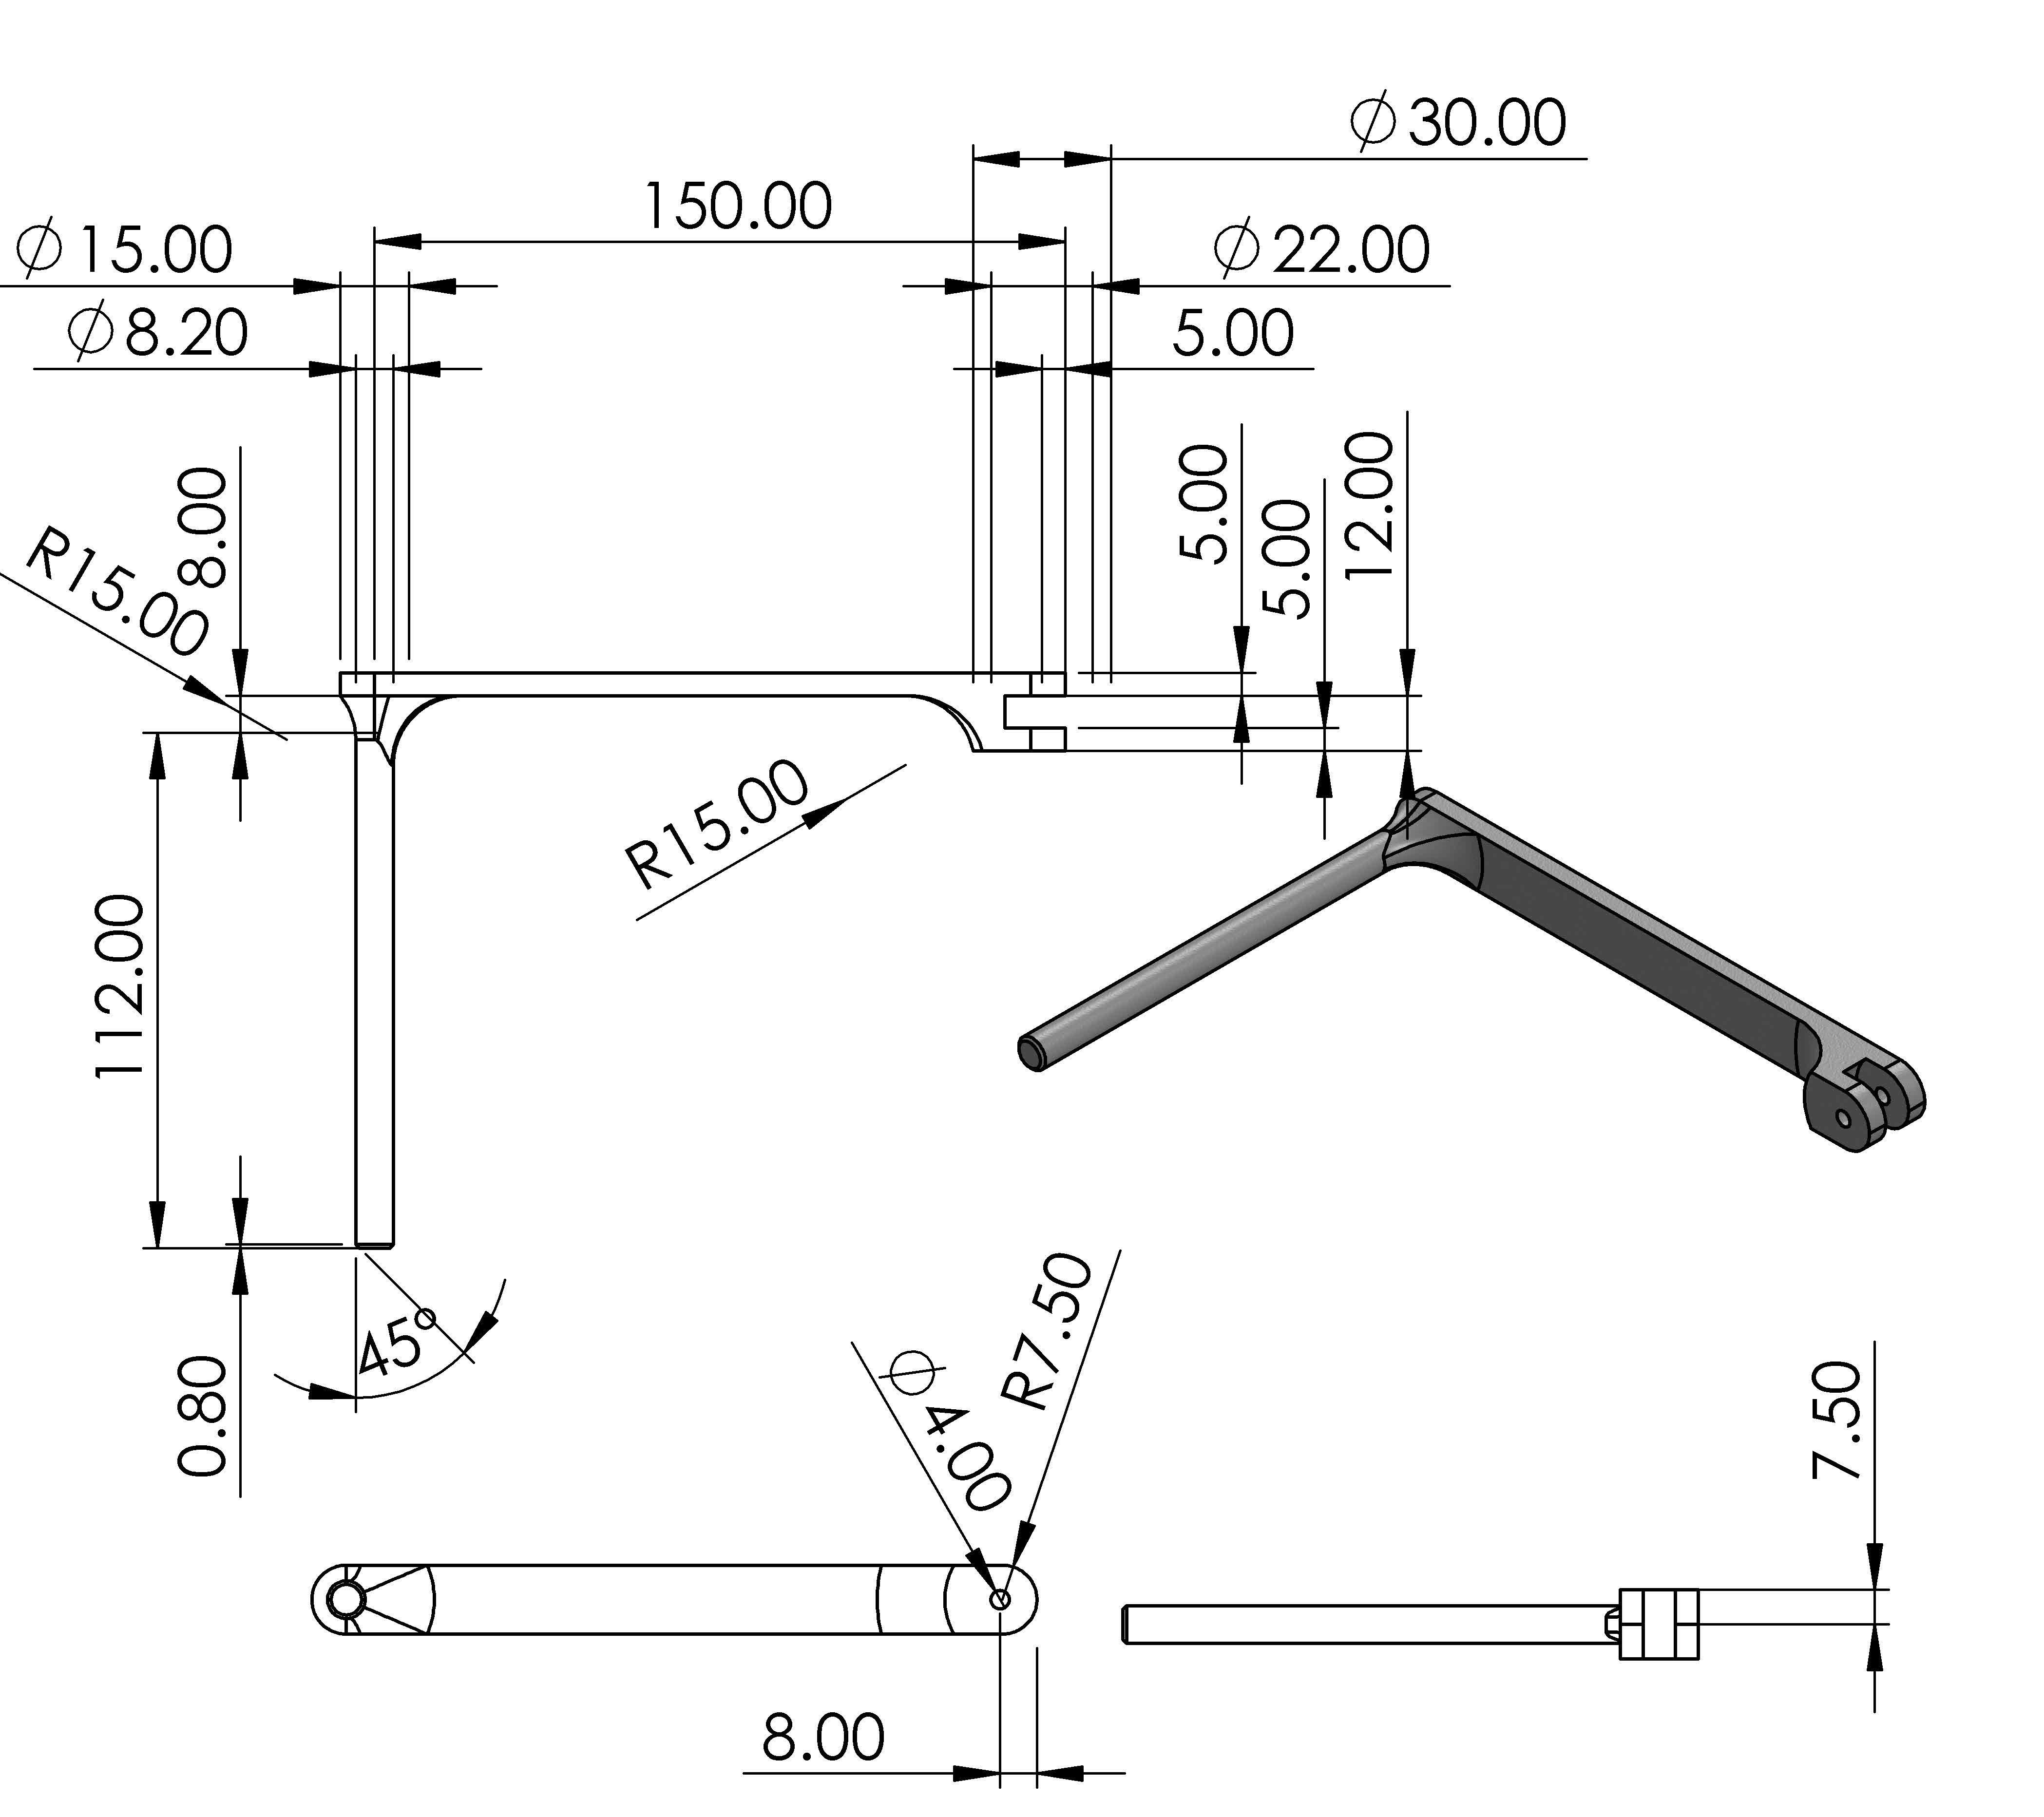
\includegraphics {Figures/RockerLink2.JPG}
\caption{Link2}
\label{fig: Link 2}
\end{figure}
\end{itemize}
\subsubsection{Electrical and Electronics}
The discharge flow control unit has two electronic components. One is the MG996R servo motor used to control the flow rate in small precise steps. The other component is the L8-T8 linear actuator used for flow diversion.
\begin{itemize}
    \item MG996R servo Motor
\par
The MG996R servo motor was initially selected for turning the ball valve in precise steps. The motor is shown in  Figure \ref{fig: 10Kg MG996R Servo Motor}
  \begin{figure}[H]
        \centering
        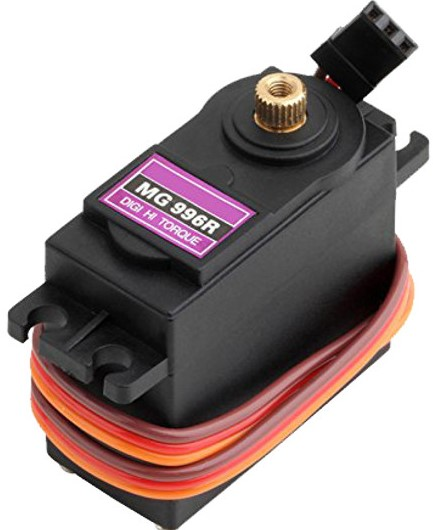
\includegraphics [height=.3\textheight] {Figures/MG996R.jpg}
        \caption{10Kg MG996R Servo Motor}
        \label{fig: 10Kg MG996R Servo Motor}
        \end{figure}
The motor has the following features;
\begin{table}[H]
\centering
\caption[MG996R Servo motor specifications]{MG996R Servo motor specifications \cite{mg996r}}
\begin{tabular}{|l|l|}
\hline
\textbf{Property} & \textbf{Value} \\ \hline
Operating Voltage & +5V \\ \hline
Current & 2.5A (6V) \\ \hline
Stall Torque & 9.4 kg/cm (at 4.8V) \\ \hline
Maximum Stall Torque & 11 kg/cm (6V) \\ \hline
Operating speed & 0.17 s/60° \\ \hline
Gear Type & Metal \\ \hline
Rotation & 0°-180° \\ \hline
Weight of motor and 55gm \\ \hline
\end{tabular}
\label{tab:MG996R_servo_specs}
\end{table}
    
From table \ref{tab:MG996R_servo_specs}, the motor's power requirement includes an operating voltage of $+5V$. This means that any voltage above 5V may be hazardous to the motor while anything below may not power the motor. The motor's electrical circuit connection is as shown in figure \ref{fig: Electrical Circuit Schematic}. From figure  \ref{fig: Electrical Circuit Schematic} a buck converter is used to stepdown the 12V DC from the main supply to the rated 6V for the motor. The ground pin was grounded onto the STM32F407 microcontroller GND pin while the pulse with modulation(PWM) pin was connected to the pin PC8 of the same microcontroller.
\par
There was however a change from the 10Kg MG996R servo motor to the DS8120 20Kg Metal Gear Digital Servo. This was because of a hinge inside the ball valve. The MG996R servo did not have enough torque to turn the valve past the hinge. Figure \ref{fig: 20Kg Metal Gear Digital Servo} shows the diagrammatic representation of the servo motor.
\begin{figure}[H]
\centering
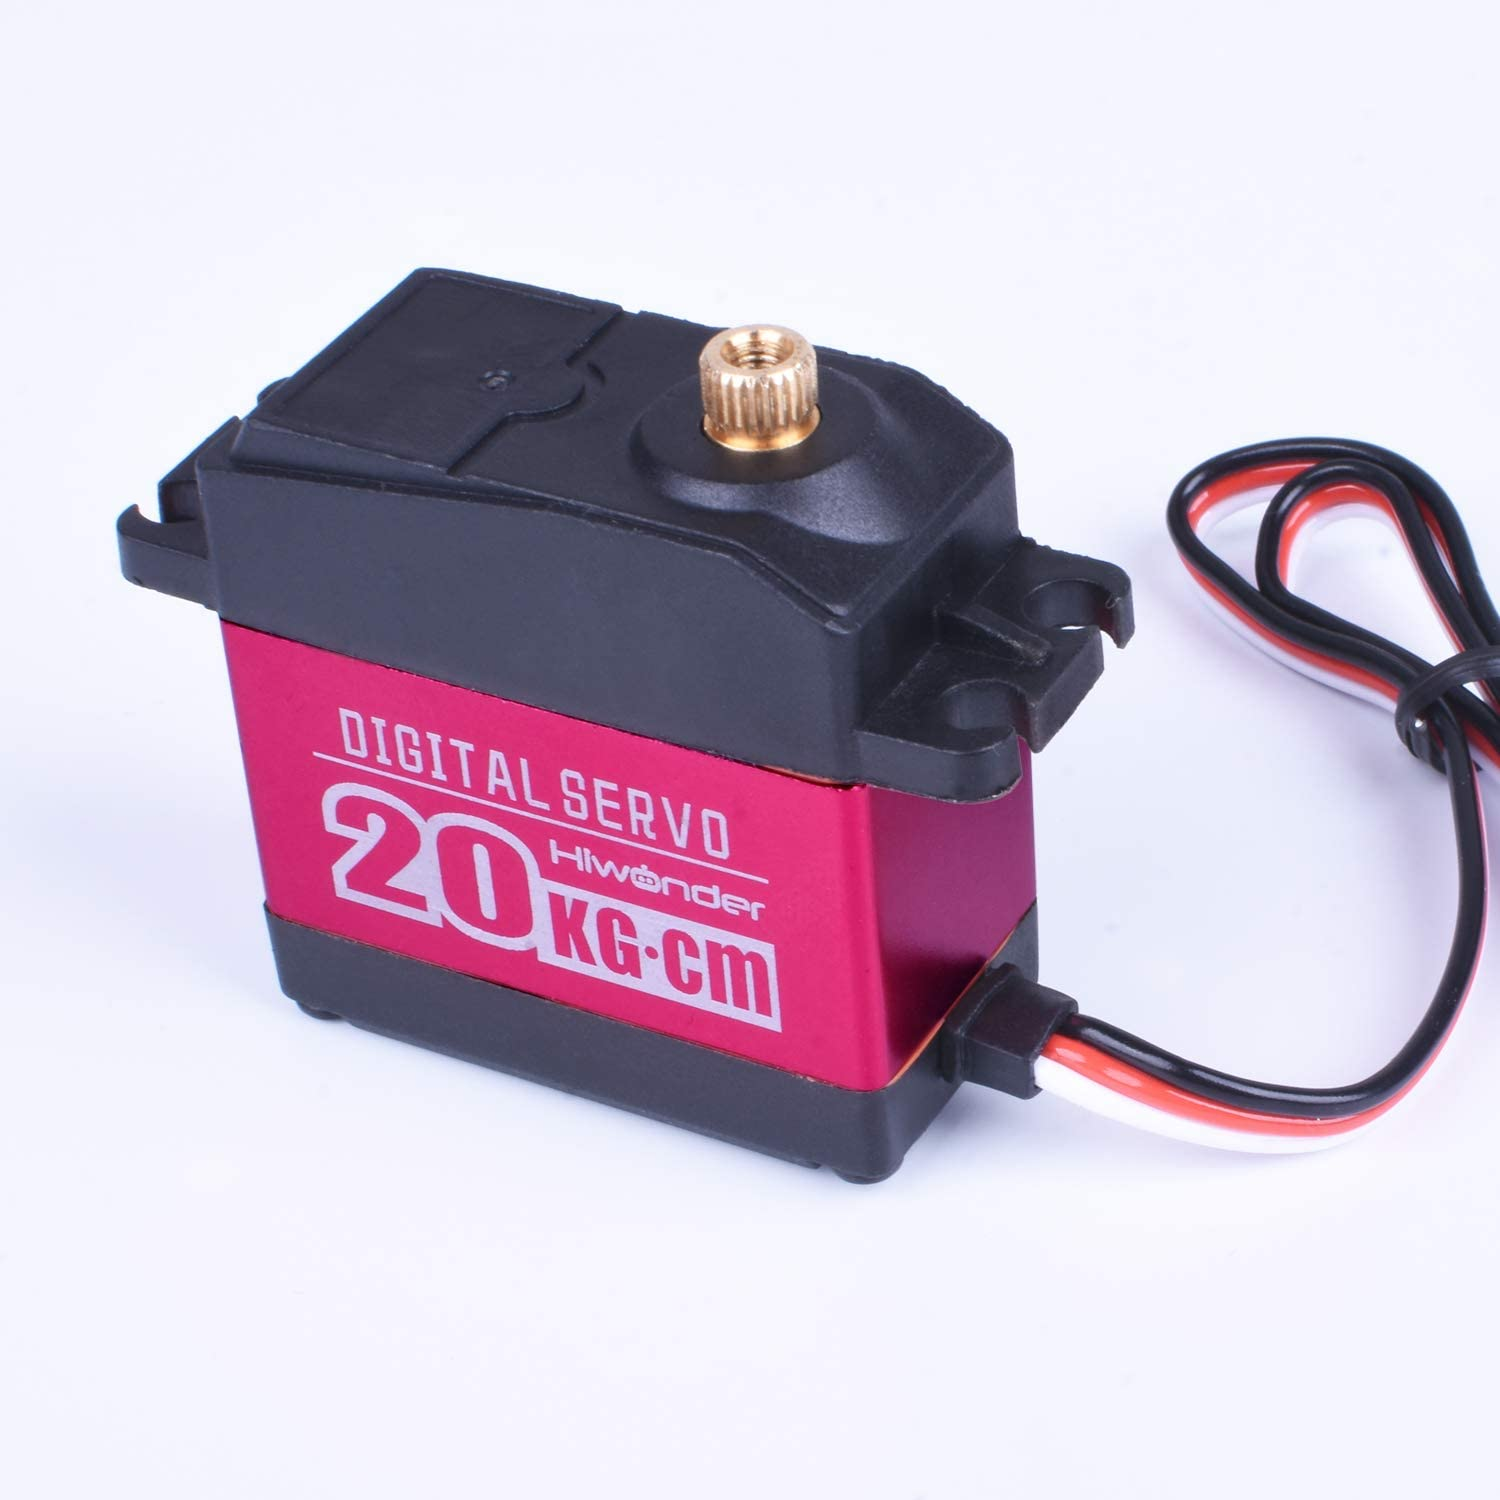
\includegraphics [height=.3\textheight]{Figures/20kg servo.jpg}
\caption{20Kg Metal Gear Digital Servo}
\label{fig: 20Kg Metal Gear Digital Servo}
\end{figure}

\begin{table}[H]
\centering
\caption[DS8120 Servo motor specifications]{MG996R Servo motor specifications \cite{d8120}}
\begin{tabular}{|l|l|}
\hline
\textbf{Property} & \textbf{Value} \\ \hline
Operating Voltage & 4.8V-6.6AV \\ \hline
Current & 2.5A (6V) \\ \hline
Stall Torque & 18.5 kg/cm (at 4.8V) \\ \hline
Maximum Stall Torque & 20.5A kg/cm (6V) \\ \hline
Operating speed & 0.17 s/60° \\ \hline
Gear Type & Metal \\ \hline
Rotation & 0°-180° \\ \hline
Weight of motor & 60gm \\ \hline
\end{tabular}
\label{tab:DS8120_servo_specs}
\end{table}
The properties of the DS8120 are shown figure \ref{tab:DS8120_servo_specs}. It has similar external dimensions as the MG996R, this therefore did not necessitate any redesign in the motor bracket.
\item \textbf{LA-T8 Electromagnet Actuator}
The LA-T8 electromagnet linear actuator is used in tandem with the diversion flap to control flow diversion. The movement of the actuator coupled to the diversion flap via a link controls the flow of the discharge either into the collection tank or into the main reservoir. The actuator is as shown in figure \ref{fig: LA-T8 Electromagnet Linear Actuator}
\begin{figure}[H]
\centering
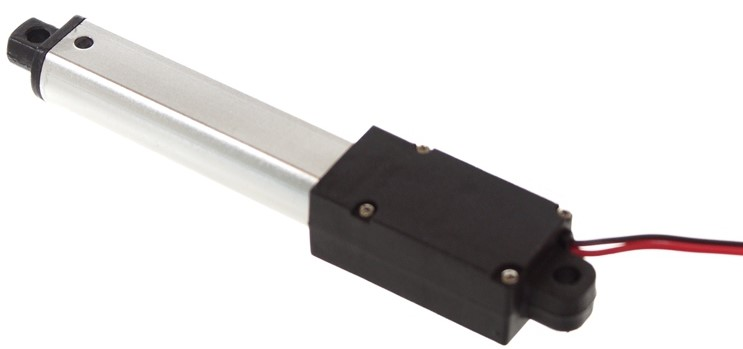
\includegraphics[height=.3\textheight]{Figures/LA-T8.jpg}
\caption[LA-T8 Electromagnet Linear Actuator]{LA-T8 Electromagnet Linear Actuator\cite{la_t8}}
\label{fig: LA-T8 Electromagnet Linear Actuator}
\end{figure}
The actuator's technical specifications are shown in table \ref{tab:LA-T8 Micro-linear Actuator technical specifications}.
\begin{table}[H]
\centering
\caption[LA-T8 Micro-linear Actuator technical specifications]{LA-T8 Micro-linear Actuator technical specifications \cite{LA-T8 Electromagnet Linear Actuator}}
\begin{tabular}{|l|l|}
\hline
\textbf{Property} & \textbf{Value} \\ \hline
Operating Voltage & 6 or 12V \\ \hline
Stroke length & 100mm \\ \hline
Stroke speed & 150mm/s \\ \hline
Maximum Load & 6.4N \\ \hline
\end{tabular}
\label{tab:LA-T8 Micro-linear Actuator technical specifications}
\end{table}
The linear actuator is connected to a 4-pole relay controlled by the microcontroller for polarity switching. The relay is connected directly from the main 12V power supply. Figure \ref{fig: Electrical Circuit Schematic} shows its electrical circuit connection.
\end{itemize}

\begin{figure}[H]
\centering
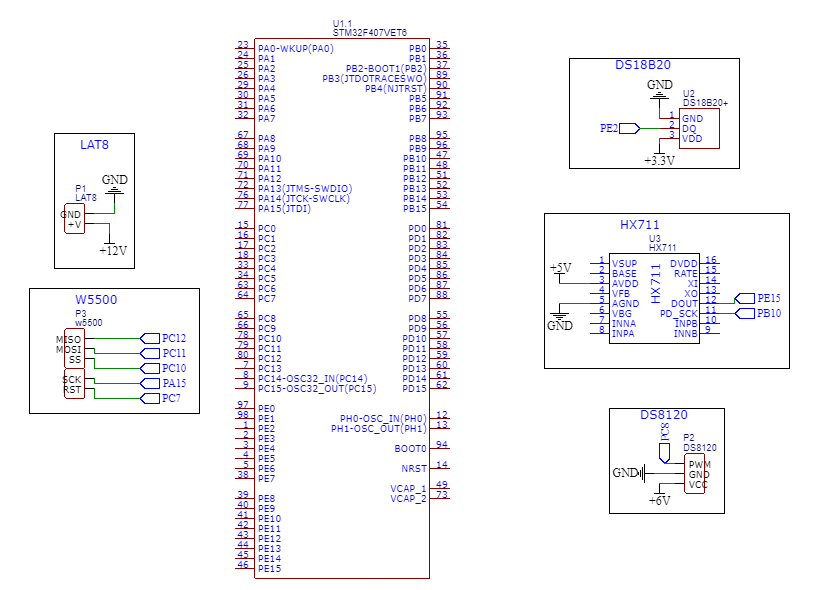
\includegraphics [width=\textwidth]{Figures/Schematic_FYP18_2022-12-10.png}
\caption{Electrical Circuit Schematic}
\label{fig: Electrical Circuit Schematic}
\end{figure}


\subsection{Discharge handling unit}

This unit collects the diverted discharge temporarily where its temperature and weight are taken. It consists of a discharge collection tank, an outlet valve, and weight and temperature measurement units.

\subsubsection{Mechanical design and fabrication}
\begin{enumerate}
    \item \textbf{Discharge collection tank}\\
        The design of the tank was based on the following considerations:
        \begin{enumerate}
            \item The shape of the tank should be such that it induces the most discharge within the shortest time possible.
            \item The tank should also be made of a material resistant to rust since it will be collecting chlorinated water.
            \item The tank should also collect not less than 20 liters. This value is obtained from previous experiments on the rig.
        \end{enumerate}
        From the above considerations, a horizontal cylindrical tank made of mild steel sheet was designed with dimensions shown in figure \ref{fig:horizontal_cylindrical_tank}. 
        \begin{figure}[H]
        \centering
        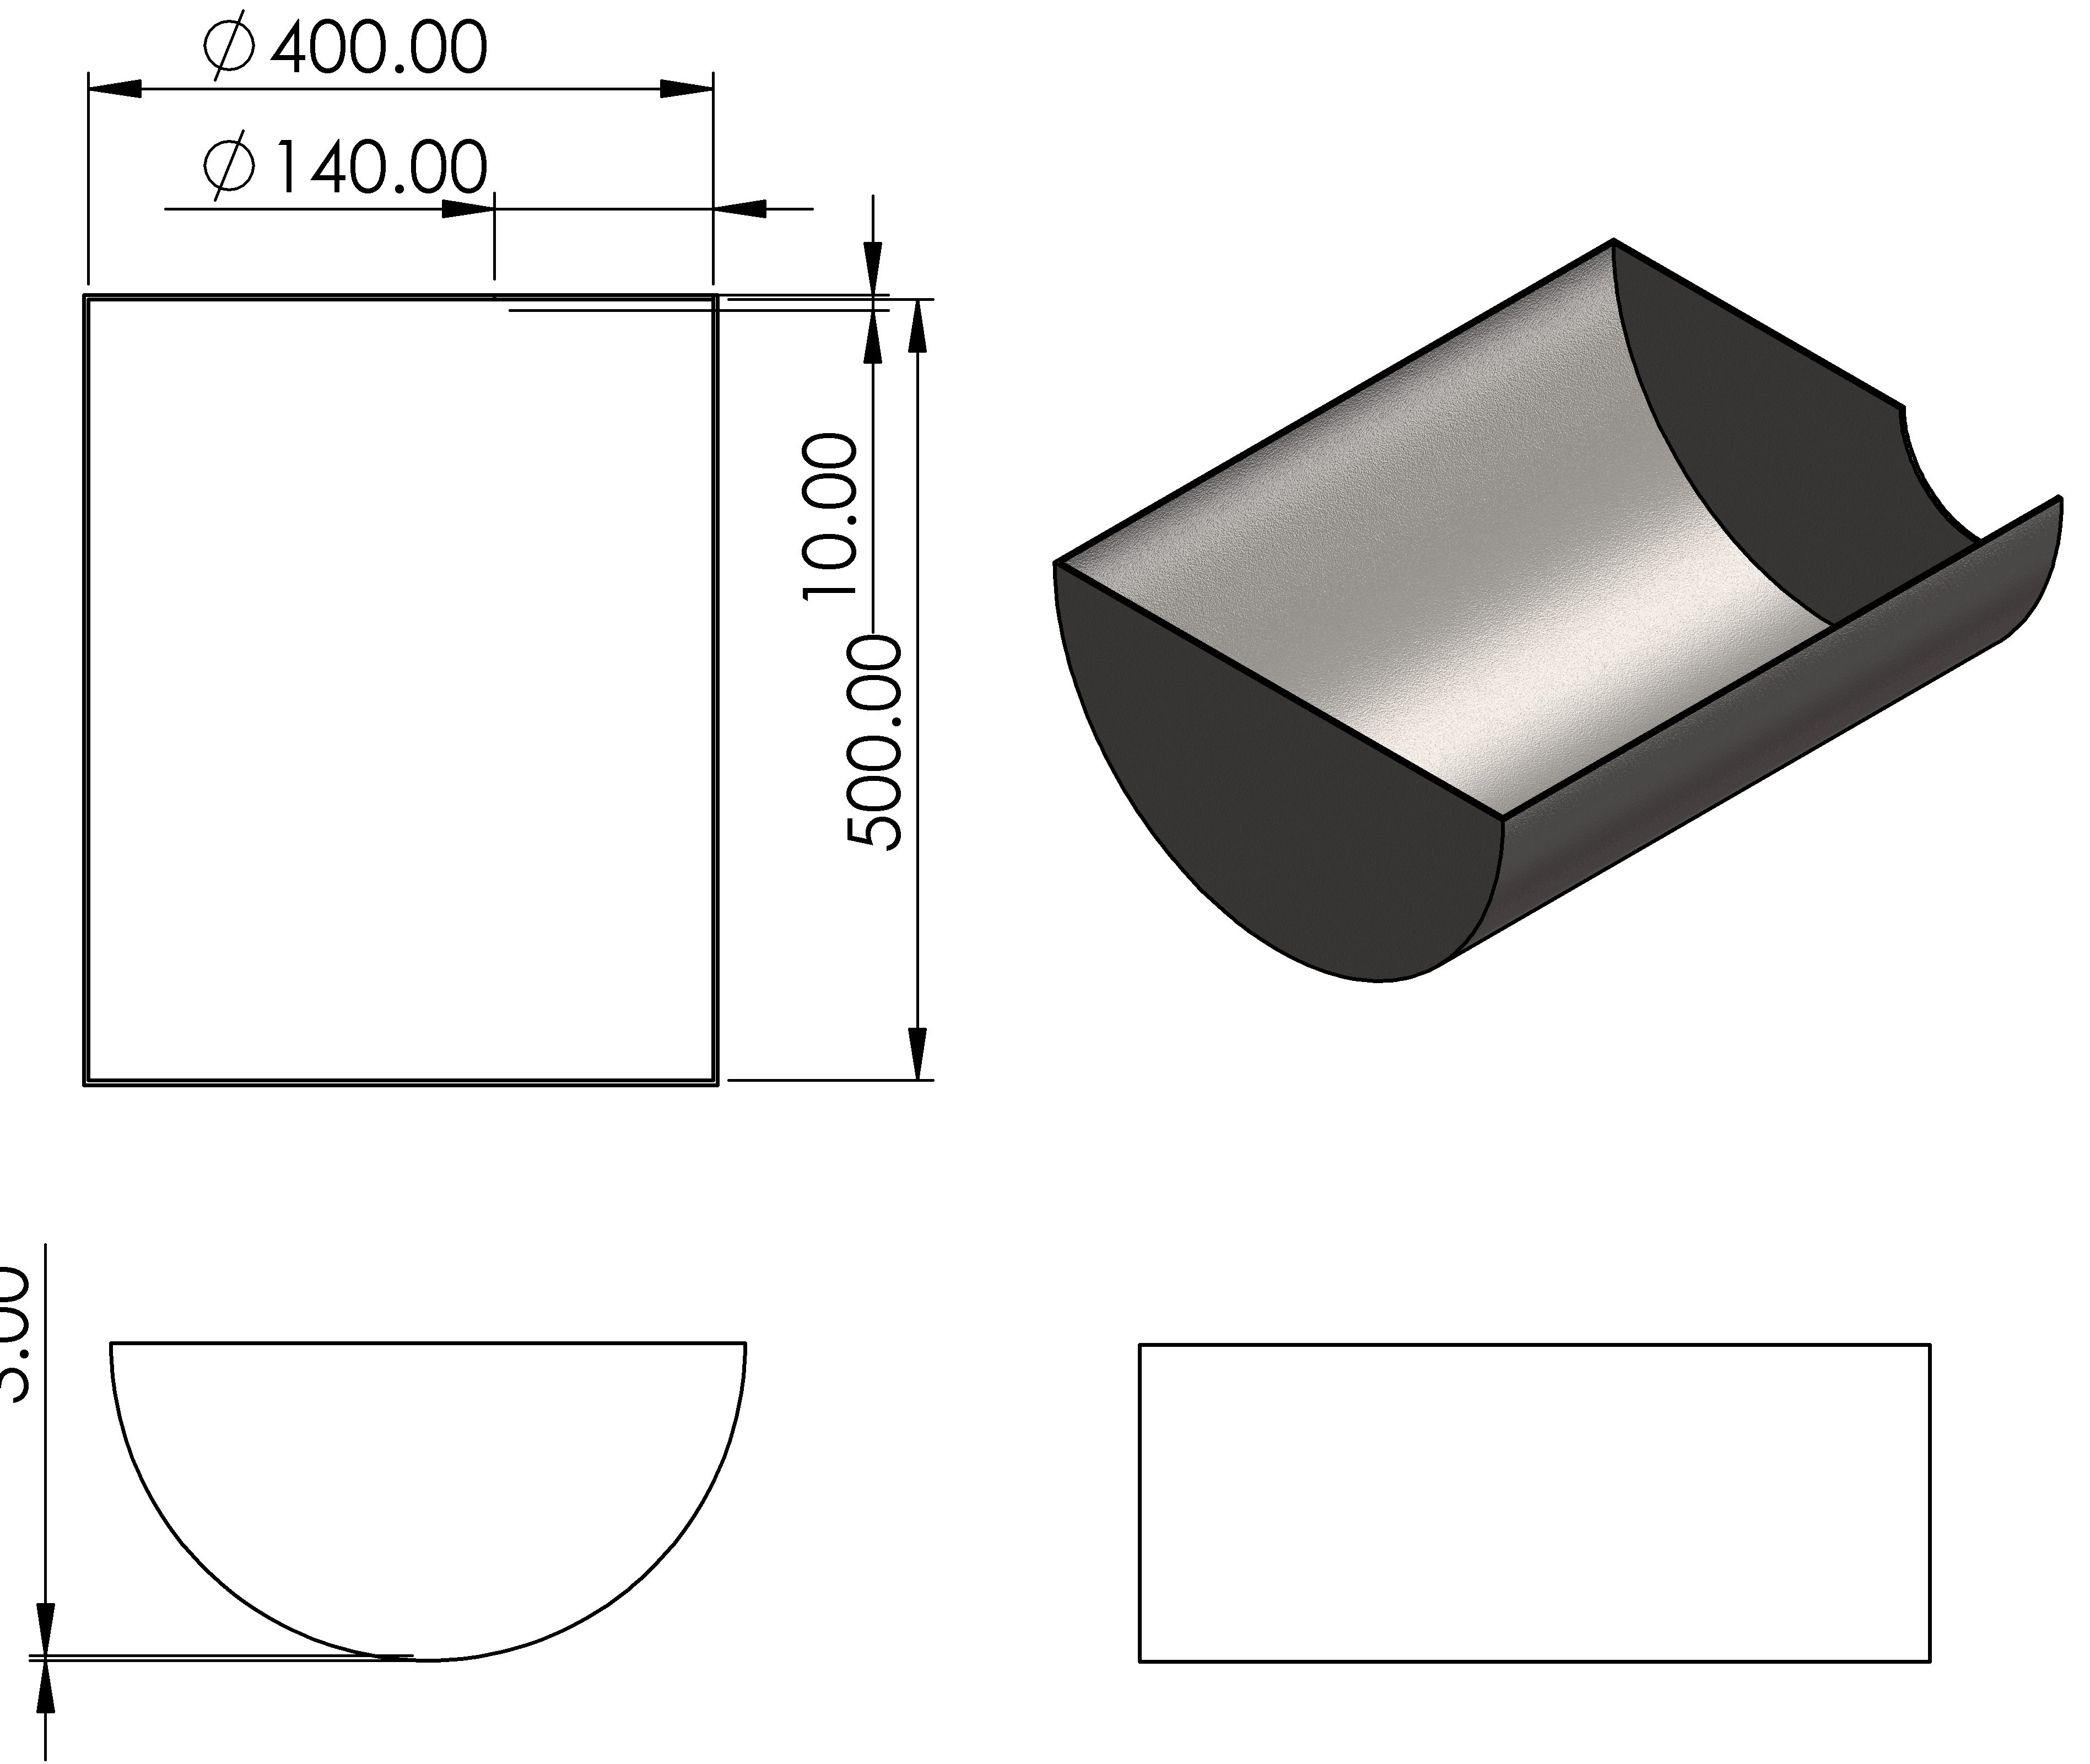
\includegraphics{Figures/tank.PNG}
        \caption{Horizontal Cylindrical tank}
        \label{fig:horizontal_cylindrical_tank}
        \end{figure}
        A support structure is necessary to support the tank. The design of the support frame is shown in figure \ref{fig:cylindrical_tank_support_frame} with its dimensions.
        \begin{figure}[H]
            \centering
            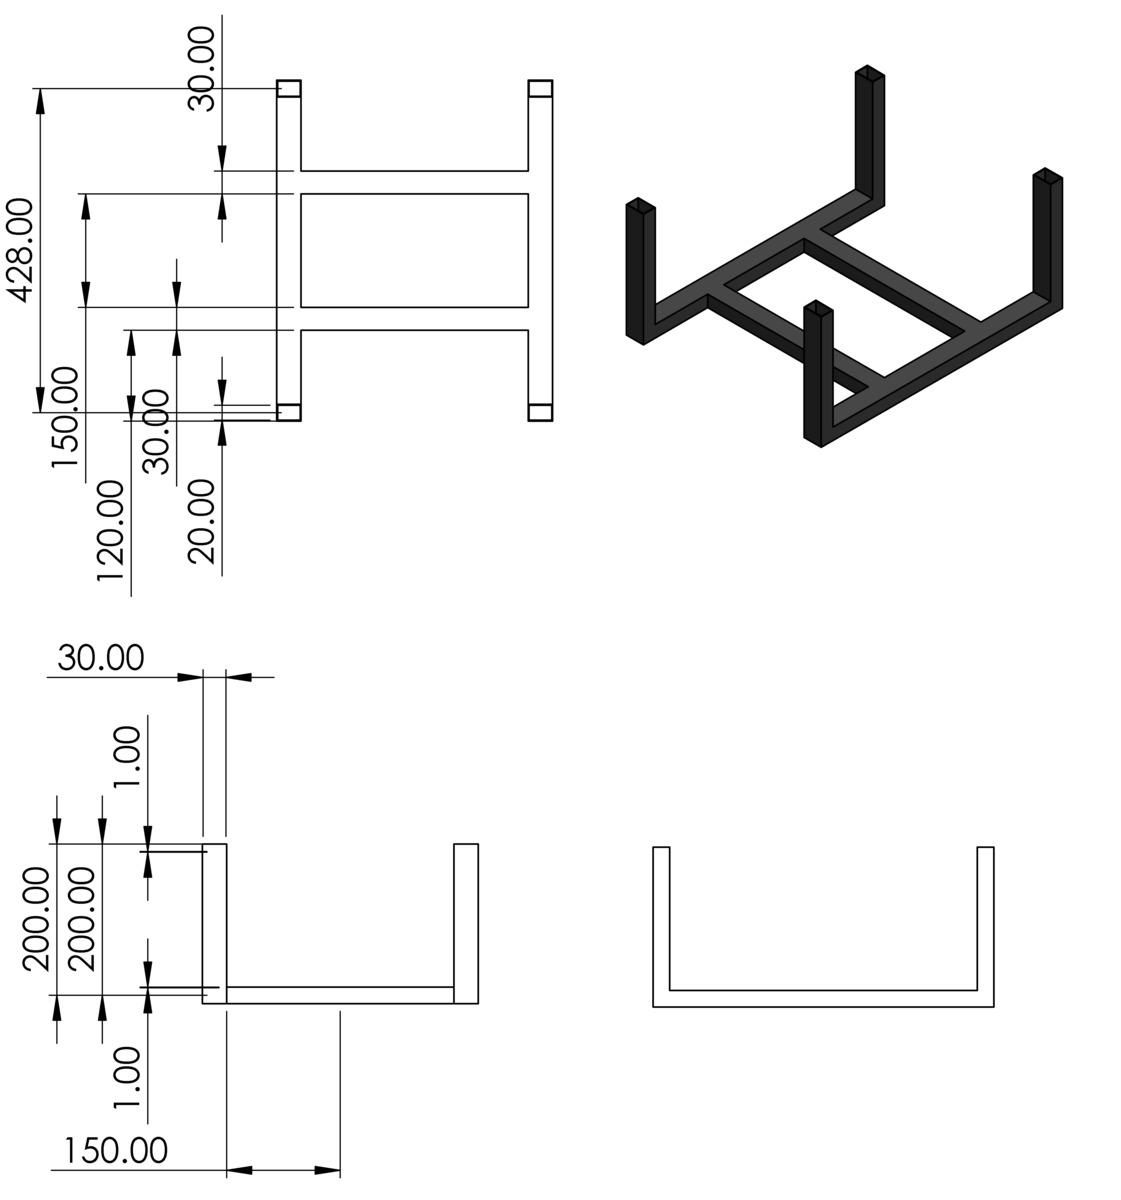
\includegraphics[height=.55\textheight]{Figures/tankHolder.jpg}
            \caption{Cylindrical tank support frame}
            \label{fig:cylindrical_tank_support_frame}
        \end{figure}
        \item \textbf{Fabrication}\\
        The fabrication of the tank started with the acquisition of $2x2$ meters of mild steel sheet. The dimensions of the sheet were obtained from the flattened sheet drawing of the tank.
        The sheet was then cut and rolled. The rolled sheets were welded together to produce the tank.
        \par
        The tank was positioned in the center of the support frame, and welded as shown in figure \ref{fig:fabricated tank}. The assembly was painted to prevent it from rusting.
        \par
        A $1\frac{1}{2} inch$ ball valve was also welded to the bottom of the tank. This size of the valve was selected such that the tank could be emptied in the least time possible. 
        \begin{figure}[H]
            \centering
            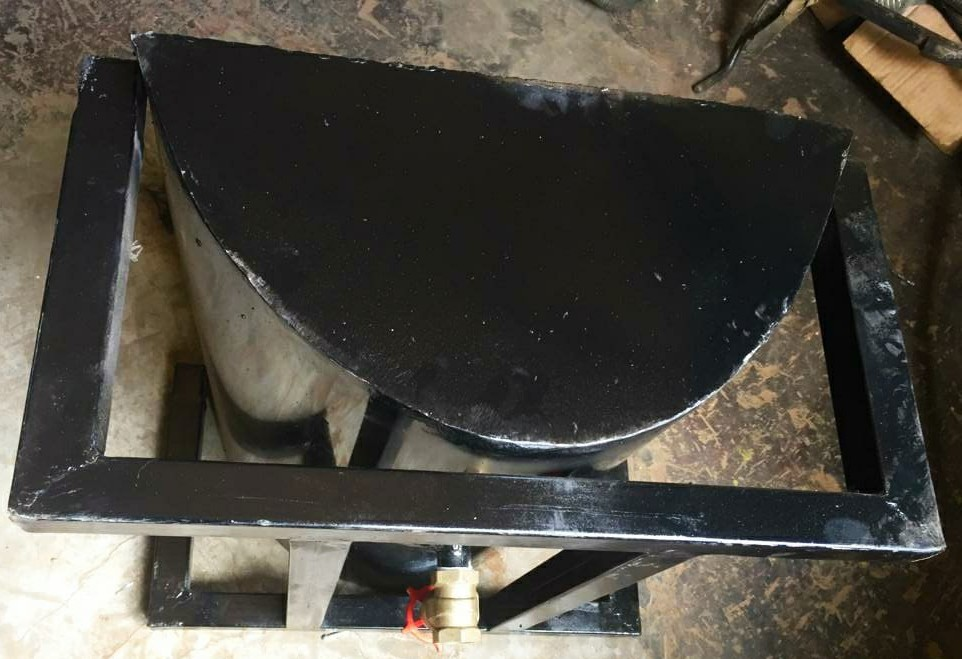
\includegraphics[width=.55\textwidth]{Figures/tank_fabricated.jpg}
            \caption{Fabricated tank}
            \label{fig:fabricated tank}
        \end{figure}
        \item \textbf{Tank support frame}\\
A support frame is necessary to support the tank and the load cells on the fluids rig right under the discharge flow control unit. The selected design of the support is shown in figure \ref{fig:tank_support_frame}. 
\begin{figure}[H]
    \centering
    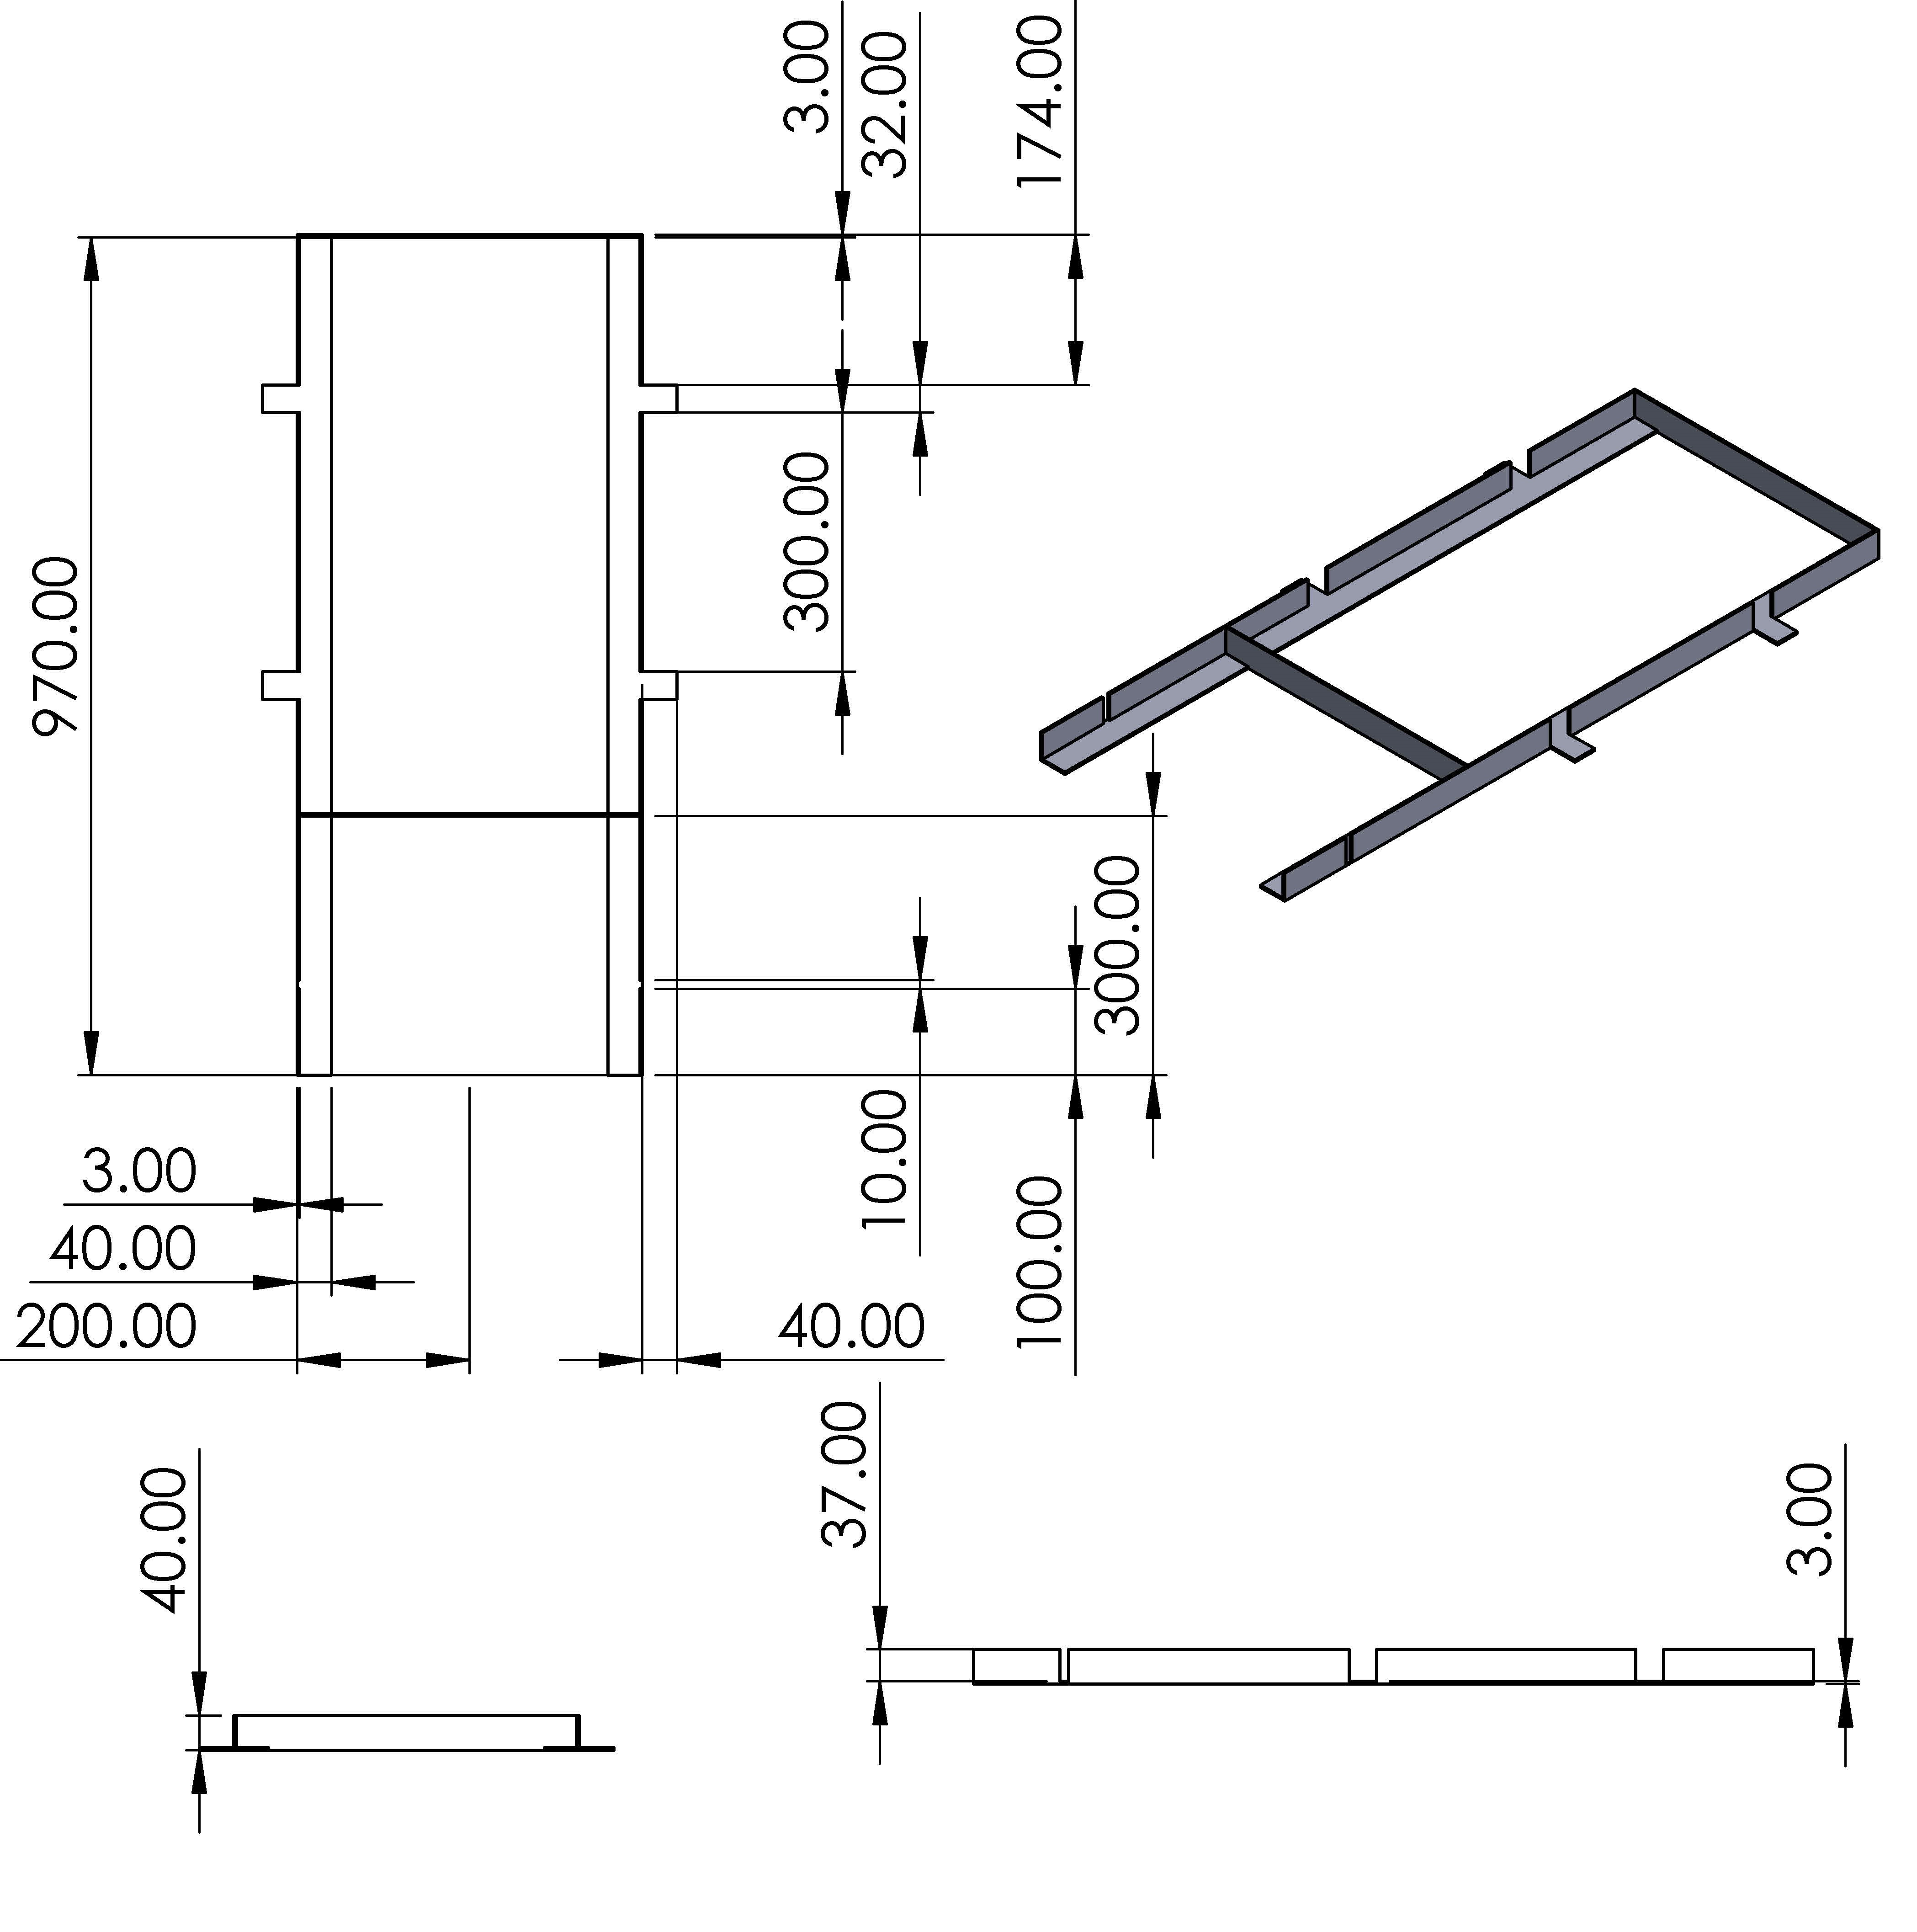
\includegraphics[height=.4\textheight]{Figures/tankSupport.JPG}
    \caption{Tank support frame}
    \label{fig:tank_support_frame}
\end{figure}
 The support frame was fabricated with $40x40 mm$ angle lines. The angle lines were cut into the sizes from the design and welded together. It was later painted to prevent it from rusting. The extension flaps on the side were slit and hammered to flatten them. This provided support for the load cells.
       \item \textbf{Cushion/suspension rubbers}\\
 For the selected load cells to perform efficiently, a pocket was made on the supporting surface to allow for the deflection of its resistive unit. Rough metallic support surface, could also provide unstable results. Therefore, a hard rubber cushion with a pocket shown in figure \ref{fig:cushion_rubber}  was designed and cut.
 \begin{figure}[H]
     \centering
     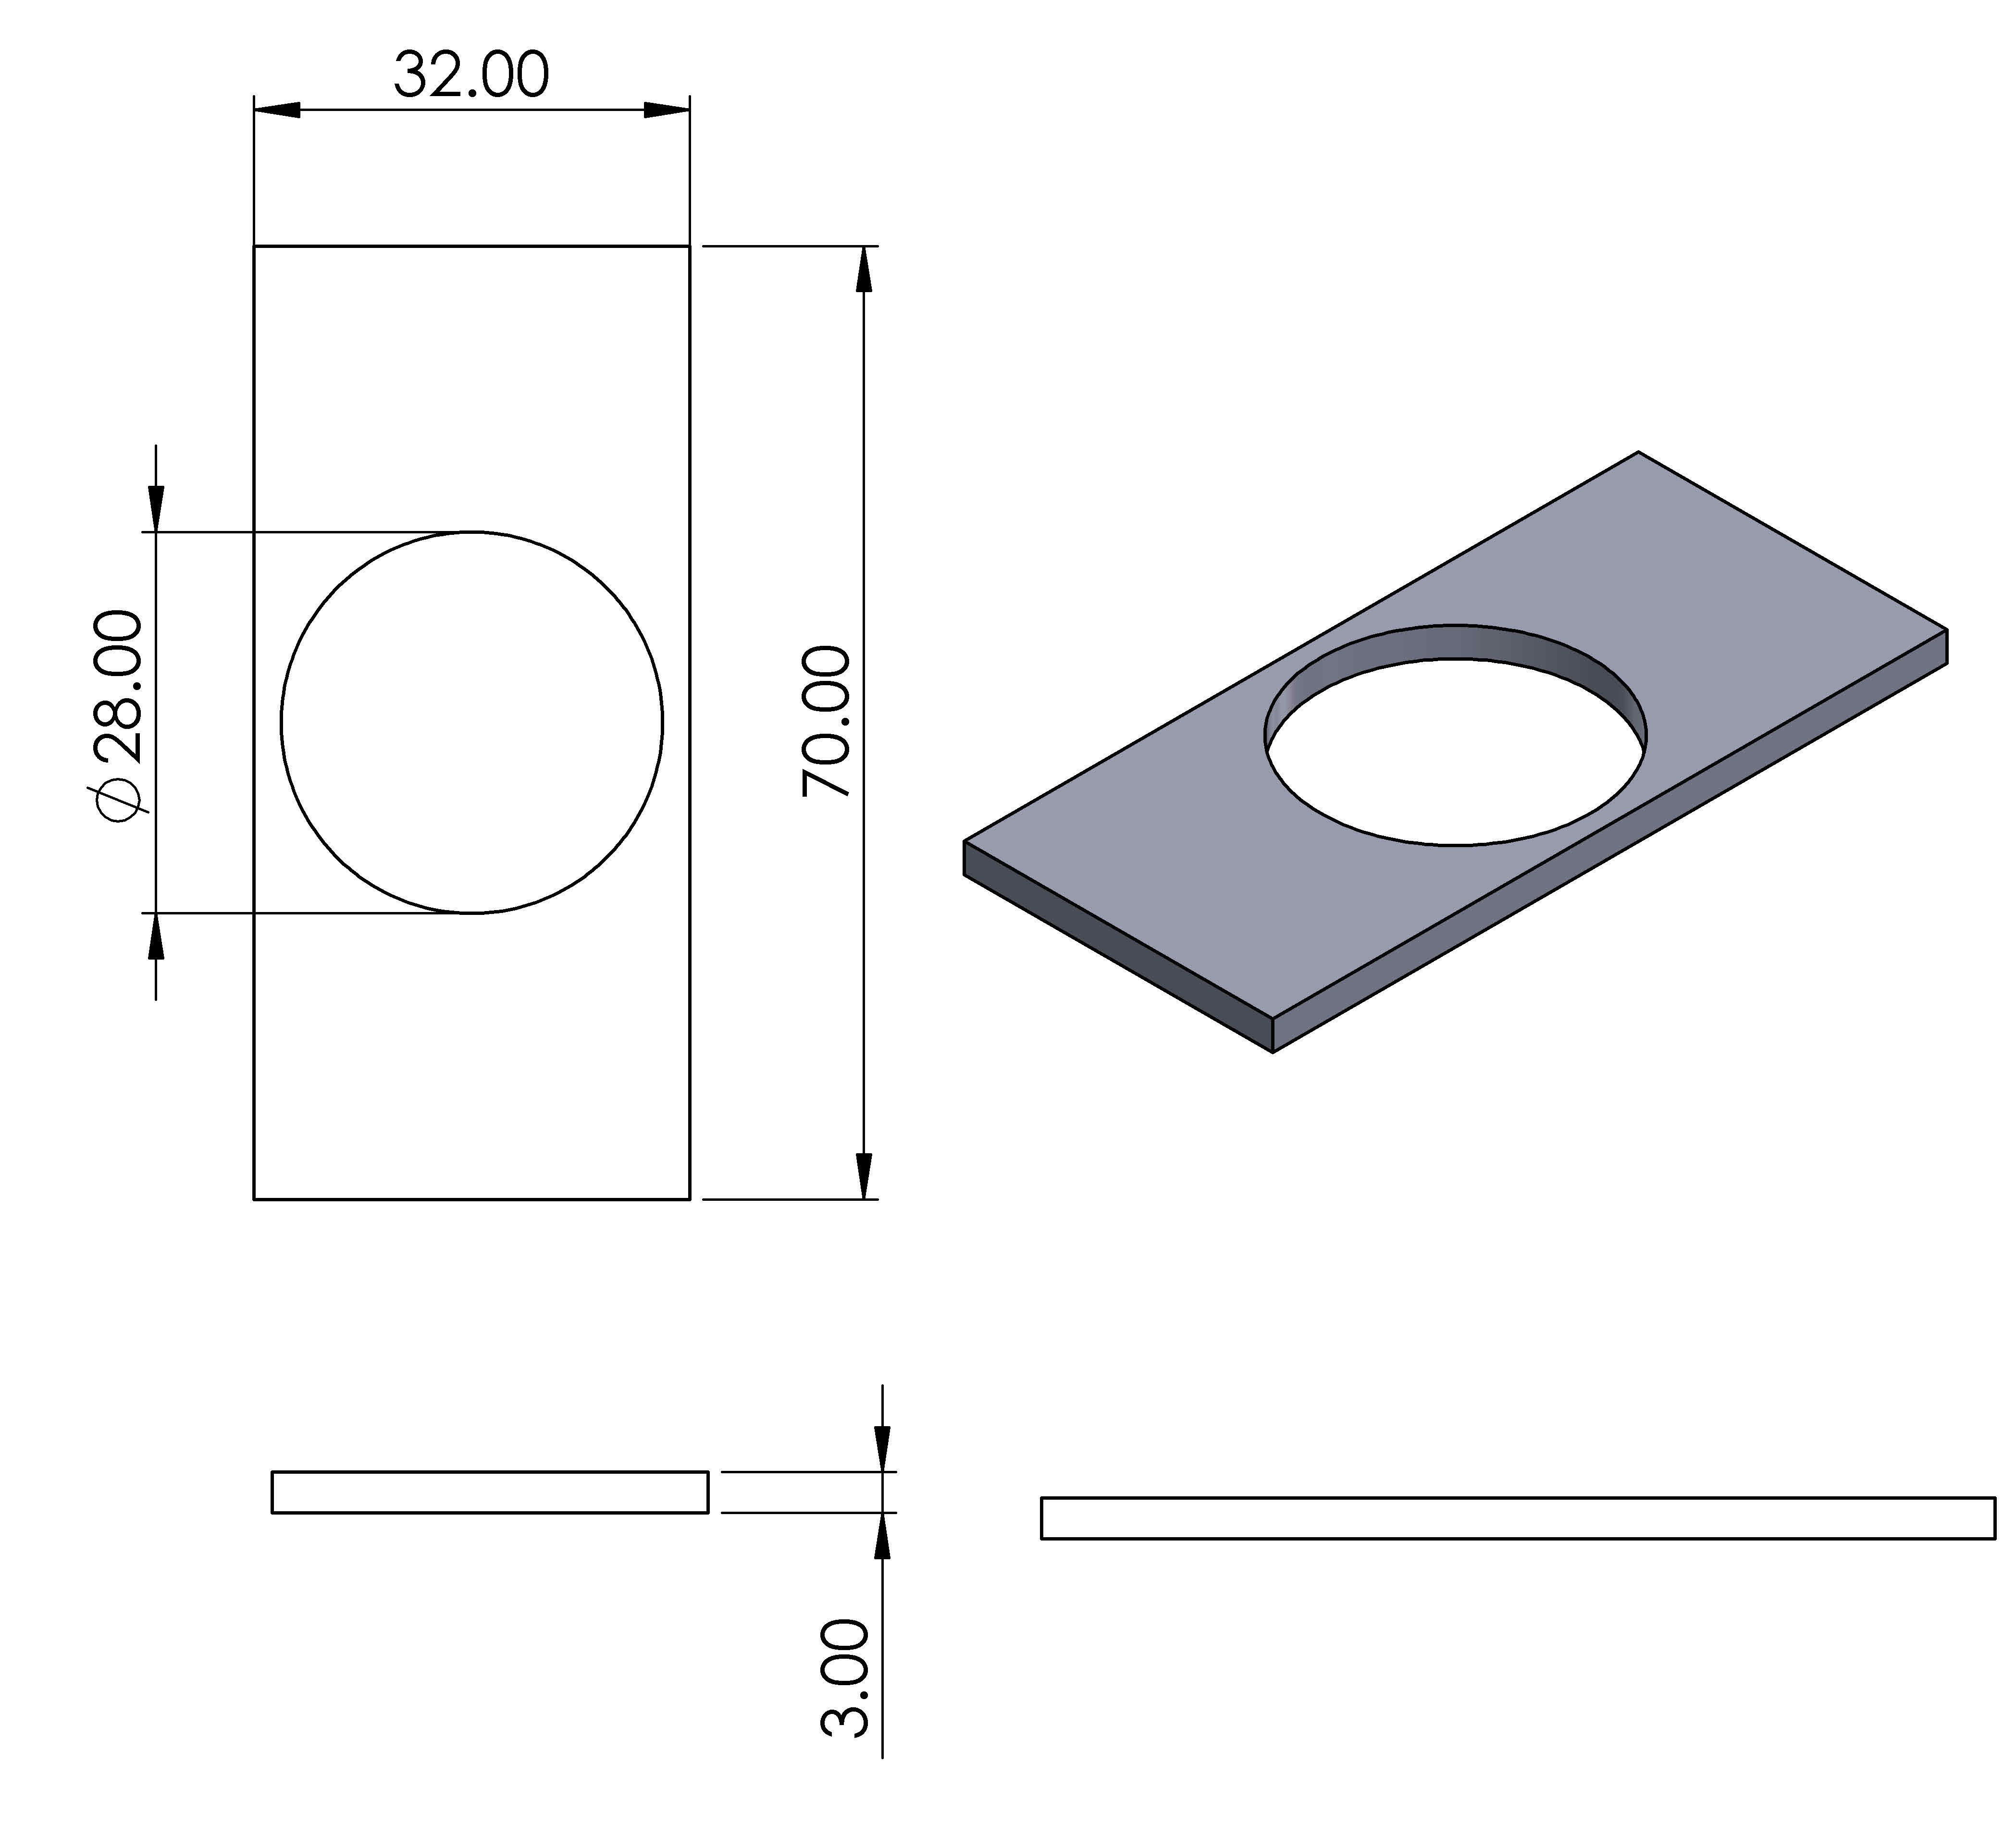
\includegraphics[width=.6\textwidth]{Figures/Rubber.JPG}
     \caption{Cushion/suspension rubber}
     \label{fig:cushion_rubber}
 \end{figure}
The rubbers are mounted between the load cells and the tank support frame as shown in figure \ref{fig:collection tank mounted}.
\begin{figure}[H]
    \centering
    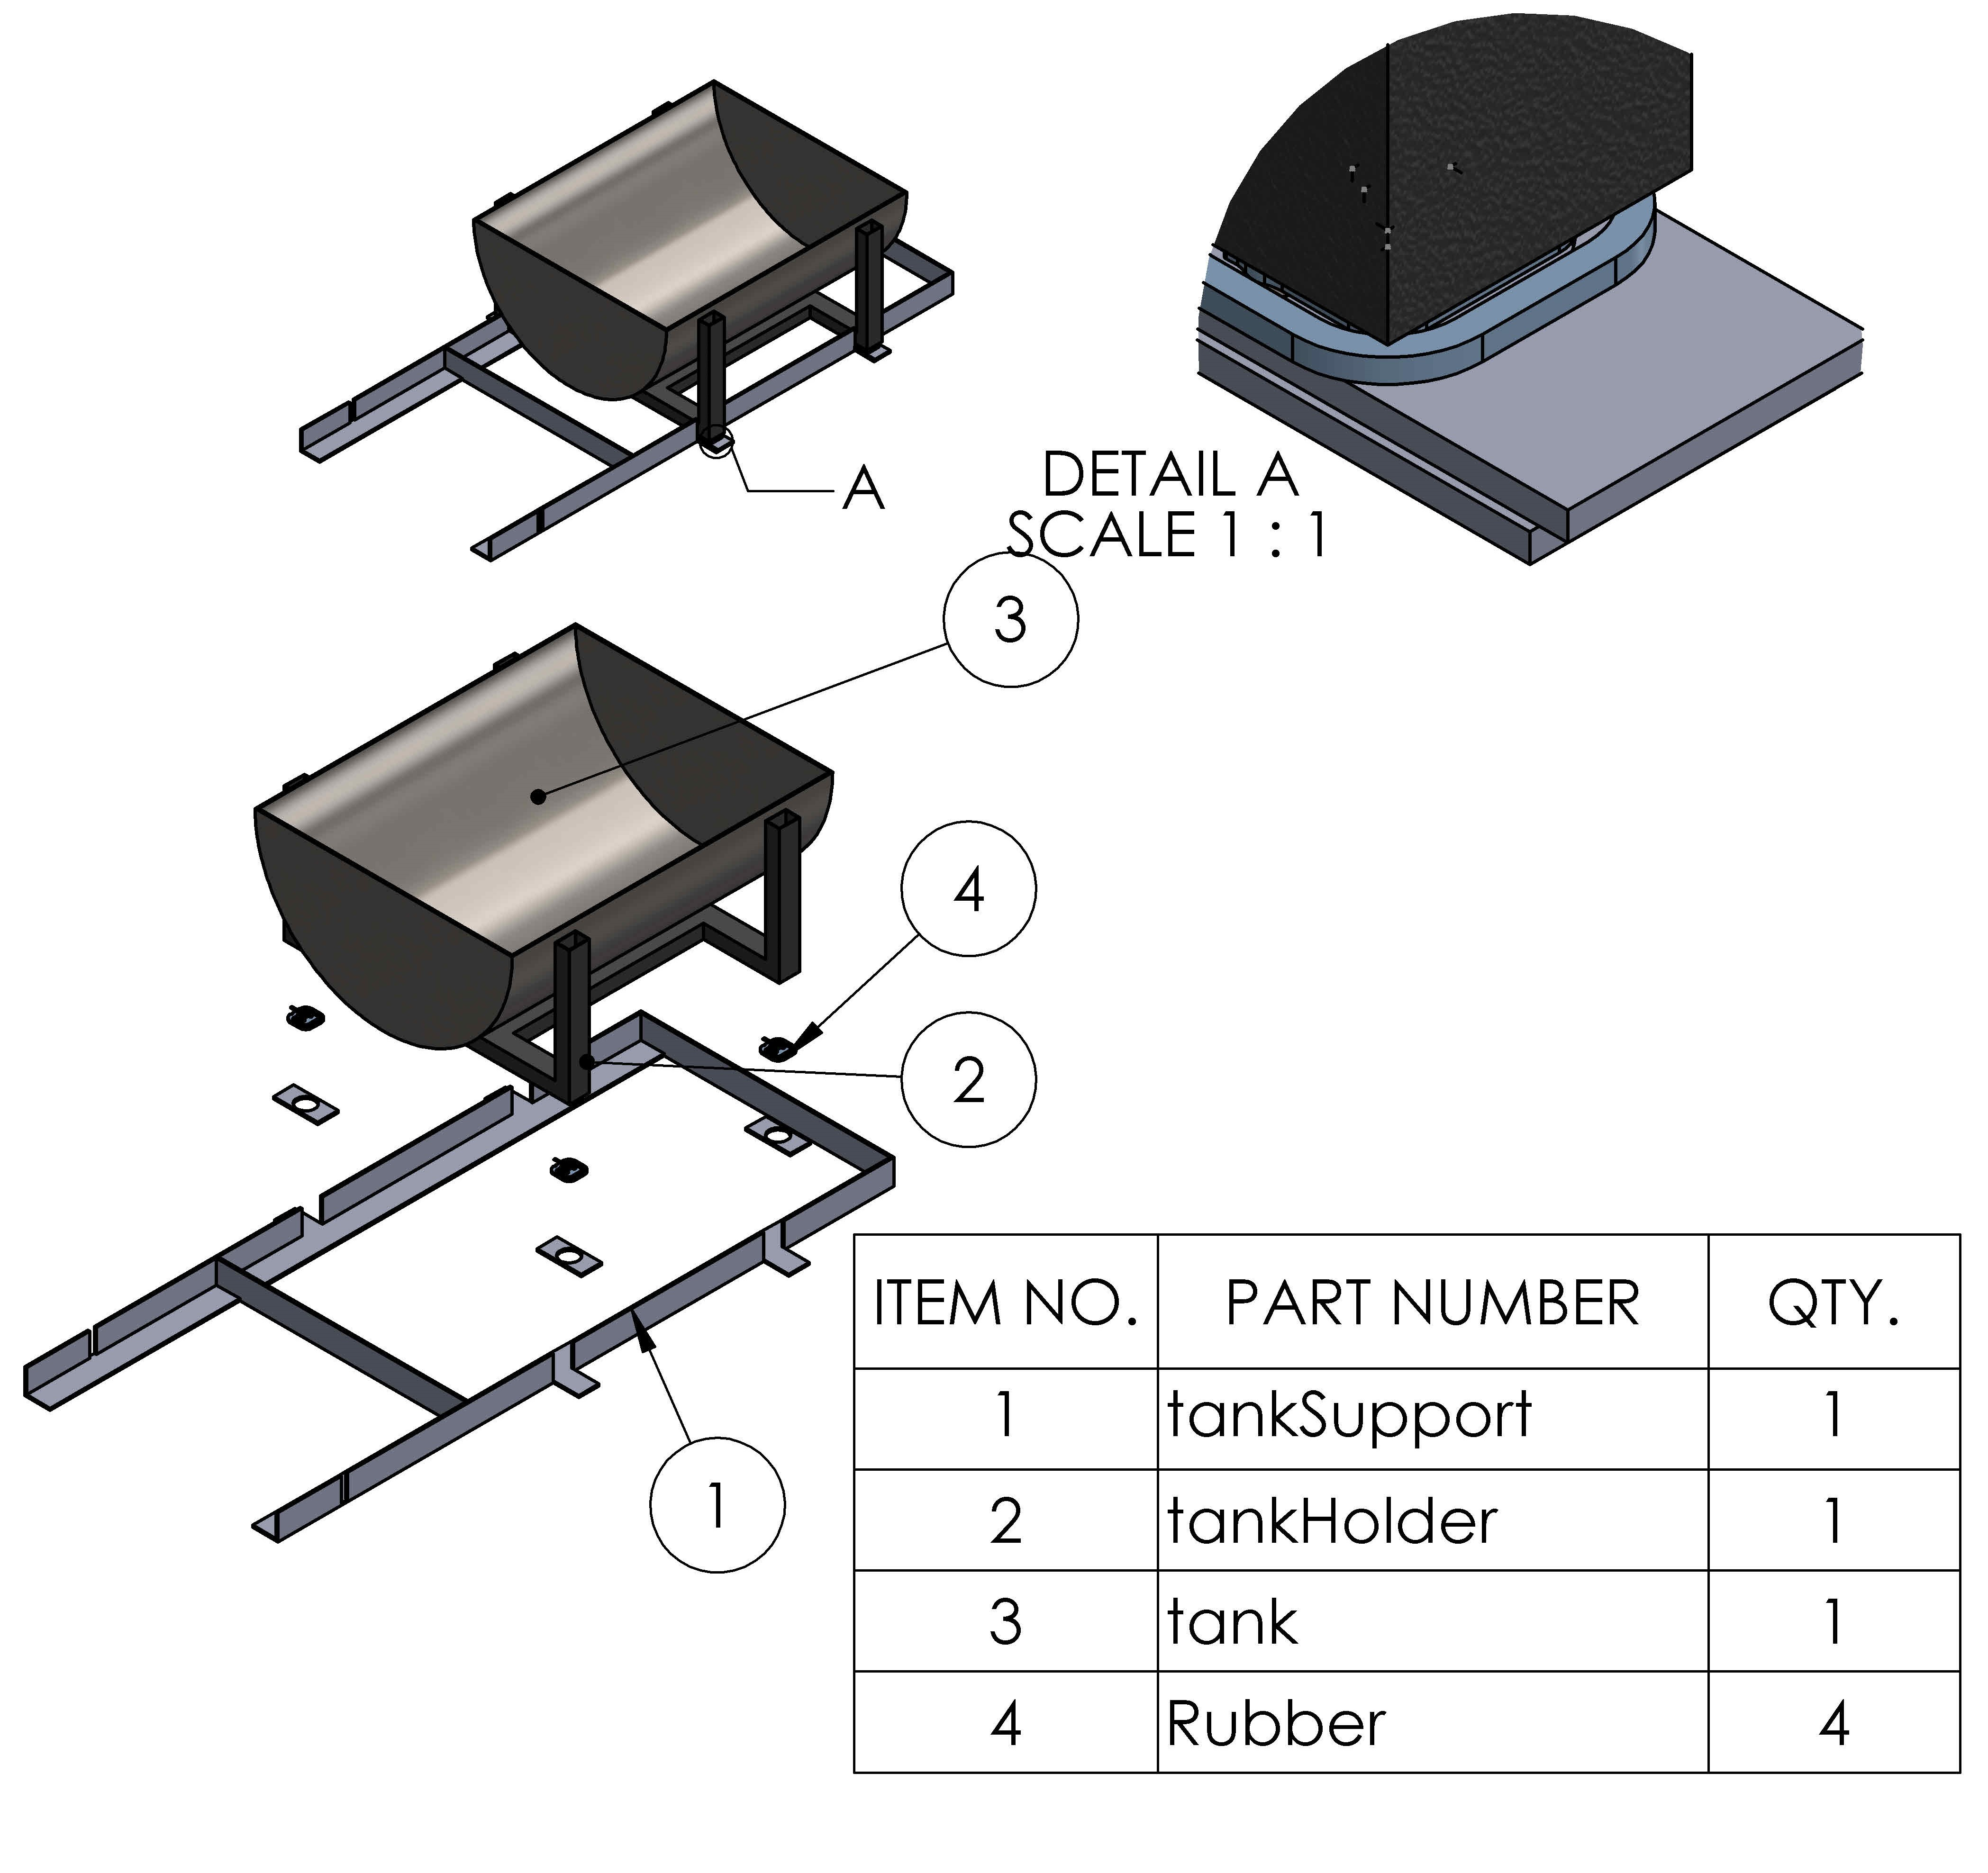
\includegraphics{Figures/CollectiontankWithSupports.JPG}
    \caption{Mounted collection tank}
    \label{fig:collection tank mounted}
\end{figure}
        \item \textbf{Plexiglass screen}\\
         A $400x400 mm$ plexi-glass piece was also cut and fitted 100 mm from the edge of the support frame in order to minimize splashes of water during an experiment.
        
\end{enumerate}  

The assembly of these parts is shown in figure \ref{fig:discharge handling unit}.
\begin{figure}[H]
 \centering
 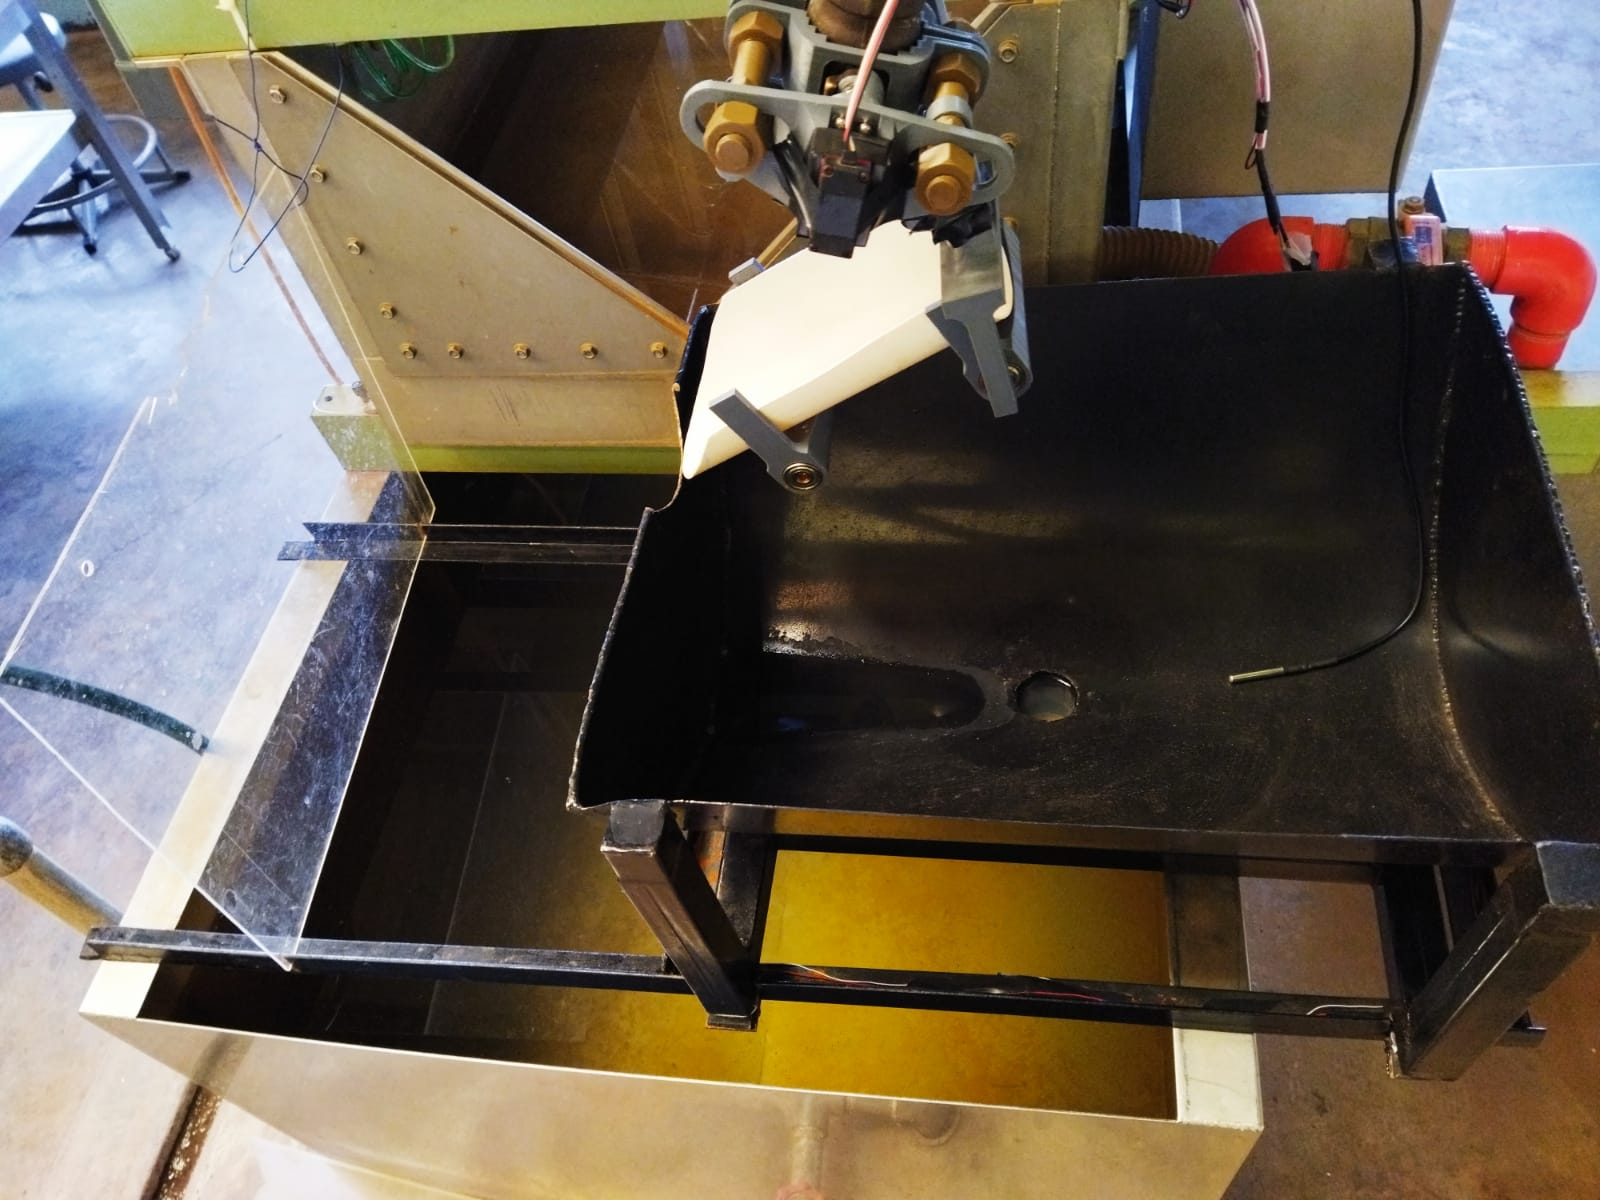
\includegraphics[width=.8\textwidth]{Figures/dsch_fabricated.jpeg}
 \caption{Fabricated discharge handling unit}
 \label{fig:discharge handling unit}
\end{figure}

\subsubsection{Electrical and electronics}
\begin{enumerate}
\item \textbf{Weight measurement unit}\\
The weight of the discharge is measured in every run of the experiment. The selection of the weight measurement sub-unit was based on the following design consideration:
\begin{enumerate}
    \item The weight in the tank is distributed to the four vertices of the support frame. This therefore necessitates four measuring units, each with a capacity not less than 20 kg.
    \item The resolution of the measuring device should be up to $\frac{1}{100}$ of a kg. 
\end{enumerate}
Based on the above considerations, four load cells each with a range of 50 kg, one of which is shown in figure \ref{fig:load_cell_disc} were selected. They are distributed to the vertices of the tank as shown in the  design in figure \ref{fig:collection_tank_with_load_cells}.

\begin{figure}[H]
    \centering
    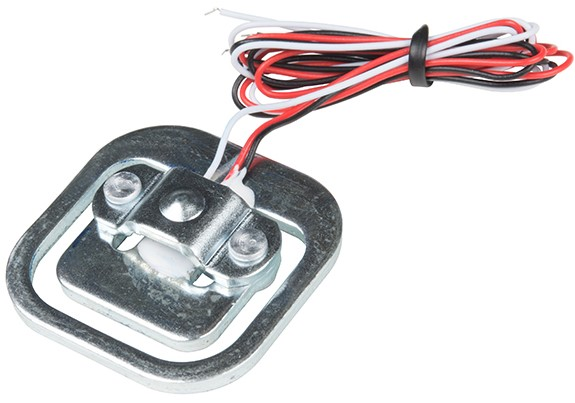
\includegraphics[width=.25\textwidth, height=.25\textheight]{Figures/50KgLoadCell.jpg}
    \caption[Strain-type load cells]{Strain-type load cells \cite{loadcell}}
    \label{fig:load_cell_disc}
\end{figure}
\begin{figure}[H]
\centering
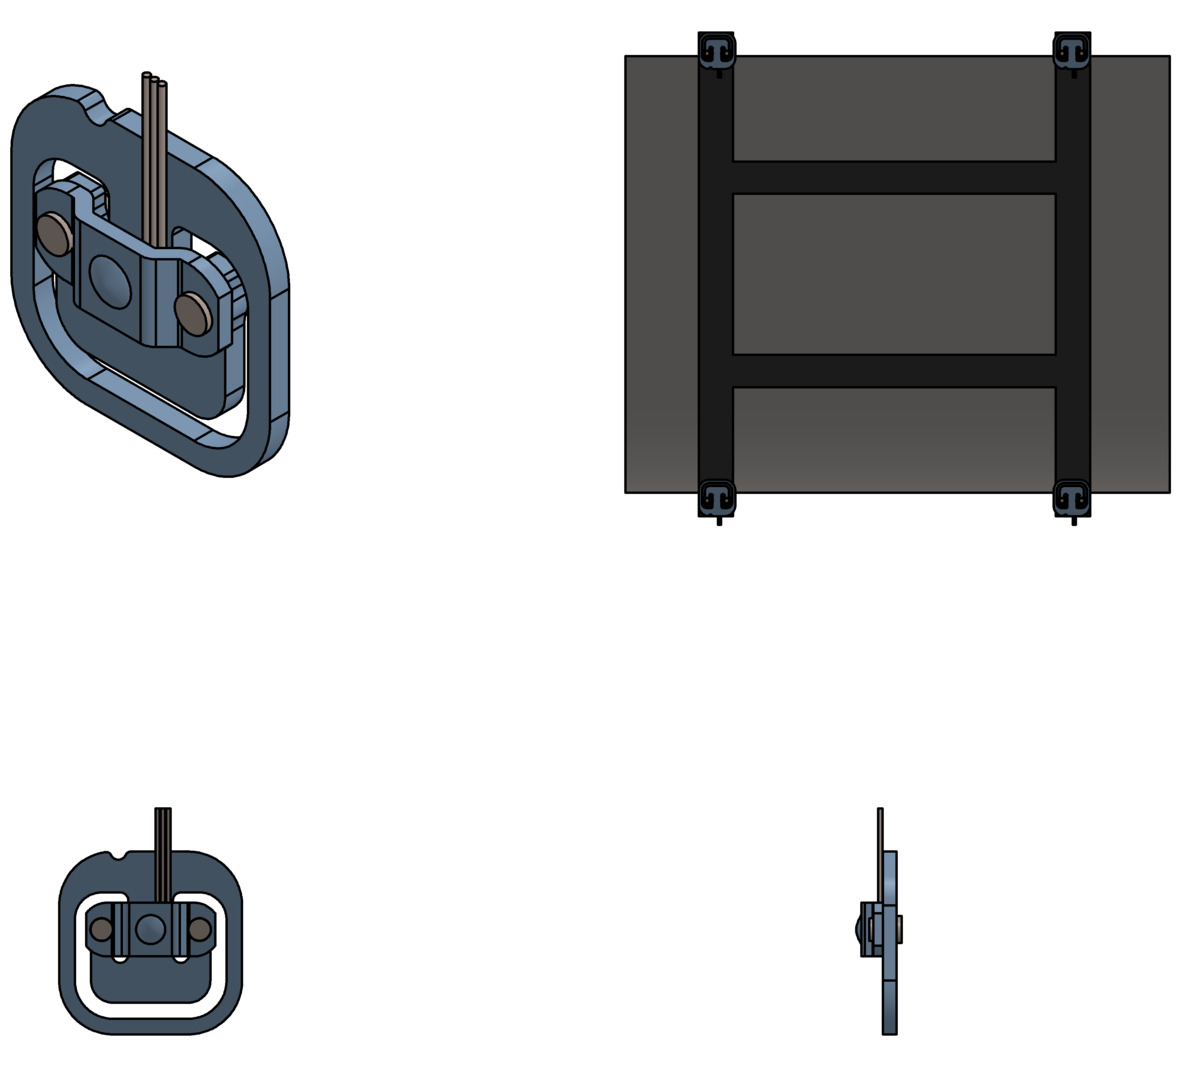
\includegraphics[height=.45\textheight]{Figures/CollectionTankWithTheLoadCells.jpg}
\caption{Collection tank with load cells}
\label{fig:collection_tank_with_load_cells}
\end{figure}

The four load cells are connected in a Wheatstone bridge as shown in figure \ref{fig:load_cell_connection}.
\begin{figure}[H]
    \centering
    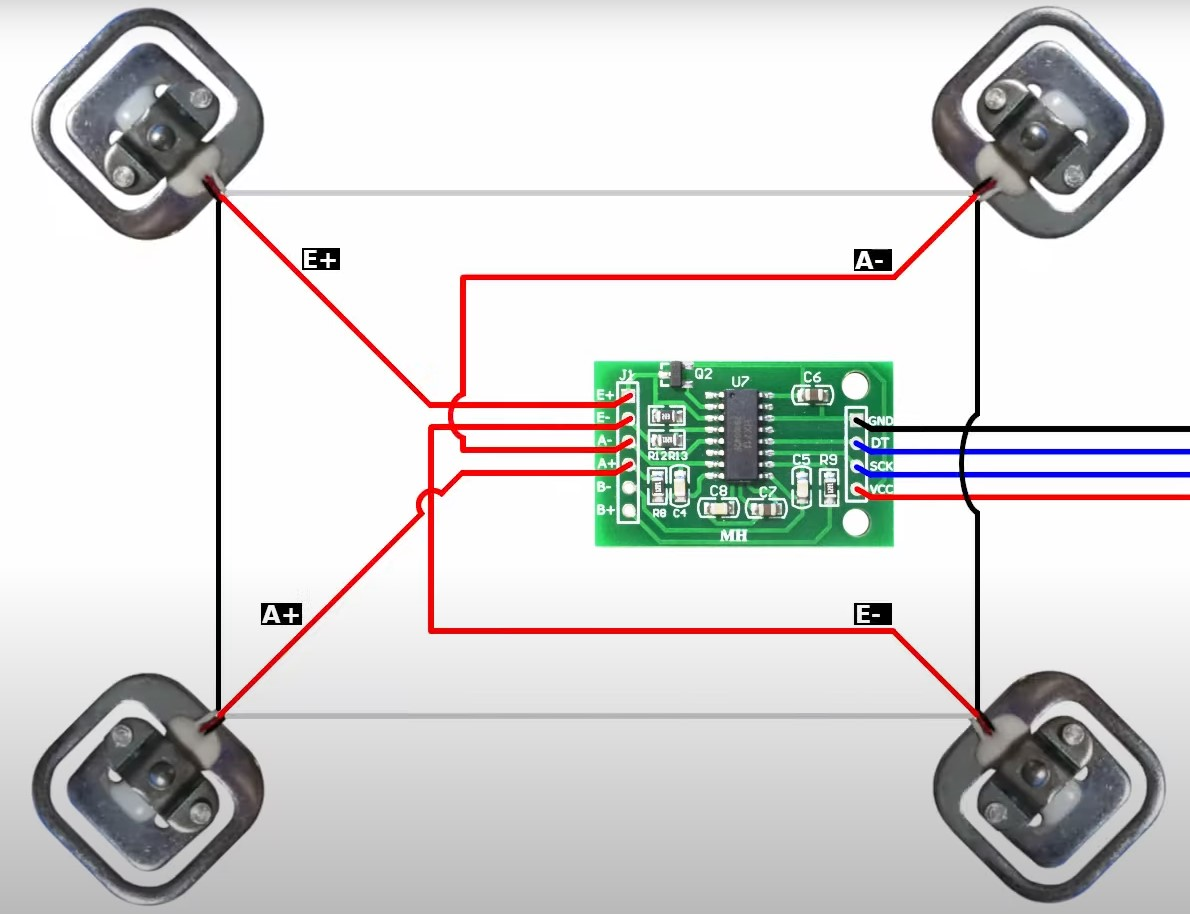
\includegraphics[width=0.45\textwidth]{Figures/LoadCellConnection.jpg}
    \caption{Load cell connection}
    \label{fig:load_cell_connection}
\end{figure}
The output of the load cells is amplified using an HX711 load amplifier which connects to an SPI interface of a microcontroller. The amplifier operates on a 5V DC supply which was provided by the microcontroller.
\item \textbf{Temperature measurement sub-unit}\\
 The temperature of the discharge is measured at every run to ensure the consistency of the data collected. Since this measurement is taken within roughly 10 seconds before the outlet valve is opened, a measuring device whose sensitivity is enough to establish reliable results within that time is required for this application. An immersible DS18B20 temperature probe shown in figure \ref{fig:ds18b20_temperature} was selected. This probe operates on a 3.3V supply supplied by the microcontroller as shown in figure \ref{fig: Electrical Circuit Schematic}.
 \begin{figure}[H]
    \centering
    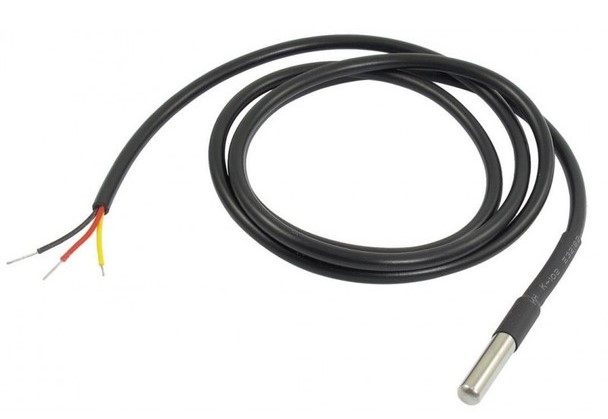
\includegraphics[width=.35\textwidth, height=.4\textheight]{Figures/ds18b20_temperature_probe.jpg}
    \caption[DS18B20 temperature probe]{DS18B20 temperature probe \cite{ds18b20}}
    \label{fig:ds18b20_temperature}
\end{figure}

\end{enumerate}
 
\subsection{Interface and control unit}
This unit consists of two sub-units:
\begin{enumerate}
    \item Interface and control sub-unit - which contains the graphical control of the system
    \item Software and controller sub-unit  - which contains the selected microcontroller for this application and firmware specifications for the application developed for the microcontroller.
\end{enumerate}
\subsubsection{Interface and control sub-unit}
It provides a means of interaction between the system and the user. Ideally, this sub-unit enables the user to input instructions and control the processes in this system. The status and results of processes in this system are also displayed in the interface. The choice of an interface depended on the following factors:
\begin{itemize}
    \item \textbf{Interface choice considerations}
    \begin{enumerate}
    \item Size \\
    This is the size of the operable part of the interface. In the case of a touch interface, a minimum of a 320x240 LCD is required to enable at least the minimum operability of GUI items, and a 20x4 LCD for any other choice.
    \item Ergonomics \\
    The user should be able to spend the least possible time feeding input and reading the results with relative ease. 
    \item Aesthetics \\
      The interface will be mostly used by students with limited exposure hence good look might be motivating. However, this should not compromise the design. It should be able to be introduced and improved with minimum modifications to the hardware in the system. 
    \end{enumerate}
     A 320x240 touch LCD interface was selected for this application. This choice satisfies all the requirements required of an interface for this application. In addition, one can also add control or  improve the aesthetics of the design by simply tweaking the GUI software without major hardware changes.

     \item \textbf{Interface Design}\\
     The interface of this application was designed with the selected electronics in mind. It included three screens:
     \begin{enumerate}
         \item \textbf{Home screen} - included all manual controls for the application.
         \item \textbf{Screen 1} - included all automated controls for carrying out a coefficient of discharge experiment.
         \item \textbf{Screen 2} - included controls for establishing wired control of the application from a remote personal computer(PC).
     \end{enumerate}
     The mock designs for this application were made in Figma online designer. The designs were then implemented using LVGL, a lightweight graphics library for embedded systems. The library is designed to run only when deployed to embedded controllers. However, a simulator can be developed on a PC for testing.
     Figure \ref{fig:home_screen} - \ref{fig:screen_2} shows the developed interfaces for this application.

     \begin{figure}[H]
         \centering
         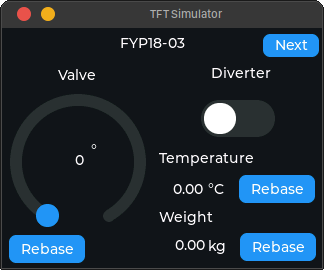
\includegraphics[width=.48\textwidth, height=.32\textheight]{Figures/home_screen.png}
         \caption{Home screen}
         \label{fig:home_screen}
     \end{figure}
     \begin{figure}[H]
         \centering
         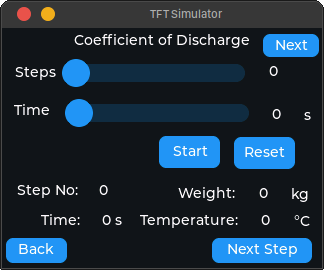
\includegraphics[width=.48\textwidth, height=.32\textheight]{Figures/screen1.png}
         \caption{Screen 1}
         \label{fig:screen_1}
     \end{figure}
     \begin{figure}[H]
         \centering
         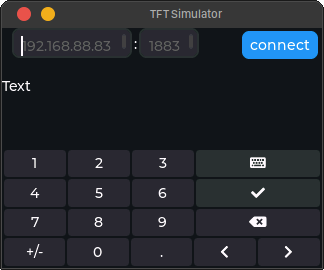
\includegraphics[width=.48\textwidth, height=.32\textheight]{Figures/screen2.png}
         \caption{Screen 2}
         \label{fig:screen_2}
     \end{figure}
     \begin{enumerate}
         \item \textbf{Home screen}\\
         The arc dial is provided for operating the valve through a servo motor in steps of $1^0$. A toggle switch is used to operate the linear actuator which in turn operates a flap that diverts a flow from the stream.
         \par
         The temperature and weight readings are continuously updated in the temperature and weight labels respectively.
         \par 
          Rebase buttons are used to reset each operation.
          \item \textbf{Screen 1}\\
          Screen 1 provides horizontal sliders for setting the number of steps and the time interval for a coefficient of discharge experiment. Clicking the start button, the value of the time and step sliders are used to compute the distribution of the operating points of the servo and the linear actuator in order to complete the experiment. 
          \par
          The reset button resets the experiment and the controls. 
          \item \textbf{Screen 2}\\
          Screen 2 provides two text fields for an IP address and the port of the connected PC. These inputs are keyed in using a virtual keyboard. The connect button initiates the business logic of establishing a connection and communicating with the PC. The virtual keyboard auto-hides. This exposes a whole text field behind where the log for the transaction between the PC and the application is displayed.
     \end{enumerate}
    \item \textbf{Application logic}\\
     The control flow of the system is shown in figure \ref{fig:control_flow}. This flow is triggered only when performing coefficient of discharge experiments. It starts when a user clicks the start button, the application then computes the control points for the valve and the diverter based on the values set for the time interval and the number of steps for the experiment. The system then turns the valve to the first control point and simultaneously initiates a timer and discharge collection. The elapsed time is continuously monitored and a different action is only taken when it elapses otherwise discharge collection continues. When the time elapses, the system stops the discharge collection and starts the temperature and weight measurement of the collected discharge. The results of the measurements are continuously updated on the graphical display. 
     \begin{figure}[H]
         \centering
         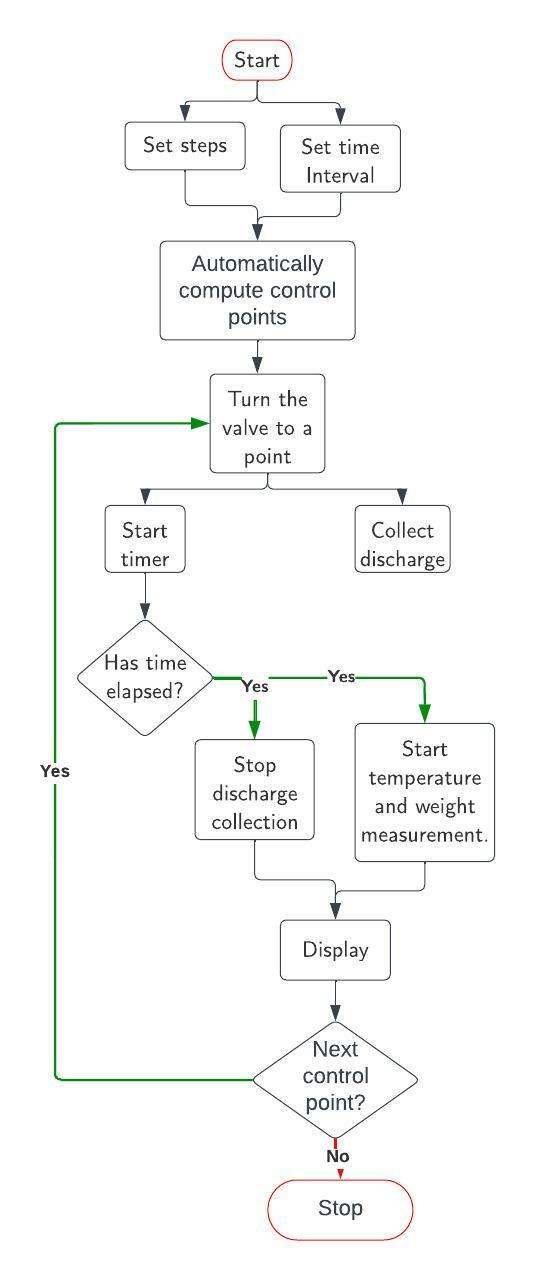
\includegraphics{Figures/Control flow.jpeg}
         \caption{Application control flow}
         \label{fig:control_flow}
     \end{figure}
     
\end{itemize}

\subsubsection{Software and controller sub-unit}
This sub-unit executes the application logic, sends instructions to the actuators, and reads inputs from sensors in the system. It is responsible for synchronizing the GUI with the processes in the hardware. Besides, it monitors and controls the parameters of the input devices and generates output signals to implement desired tasks.
\par
The selection of a micro-controller for this application was based on the following requirements:
\begin{enumerate}
    \item Support for a touch LCD screen. 32 Digital I/O pins are required in order to support a parallel 16-bit MCU Interface, and a 16-bit data bus is required for this application.
    \item Support for real-time multi-threaded firmware. This necessitates support from RTOS-operating systems. This is to allow for several threads, at least 2 threads minimum: one for handling the GUI, and another for handling the application's business logic.
\end{enumerate}

A STM32F407VET6 microcontroller board shown in figure \ref{fig:fsmc_interface} was selected for this application. It has a dedicated FSMC interface for supporting LCD touch screens. Besides, it can also support real-time multi-threaded firmware.
 \begin{figure}[H]
        \centering
        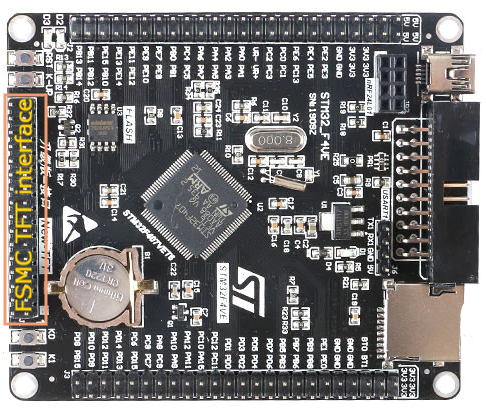
\includegraphics[width=.45\textwidth, height=.325\textheight]{Figures/STM32F407VET6.png}
        \caption[Load cells circuit]{FSMC interface in STM32F407VET6 \cite{mcu_lcd}}
        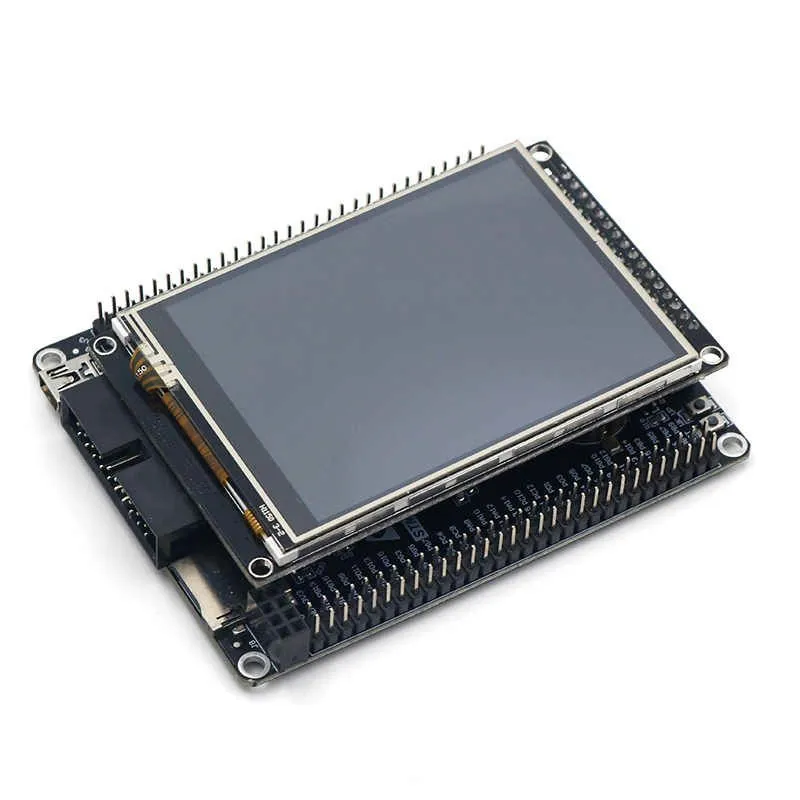
\includegraphics[width=.45\textwidth, height=.325\textheight]{Figures/stm32f407vet6_with_lcd.png}
        \caption[STM32 connected with LCD]{STM32 connected with LCD \cite{mcu_lcd}}
        \label{fig:fsmc_interface}
\end{figure}

Mbed-OS RTOS was selected for the development of the firmware for this application. It has a vast amount of APIs that simplify development and abstract the HAL code.
\begin{itemize}
    \item \textbf{Application architecture}\\
    Figure \ref{fig:firmware_architecture} shows the architecture of the firmware for this application.
    \begin{figure}[H]
        \centering
        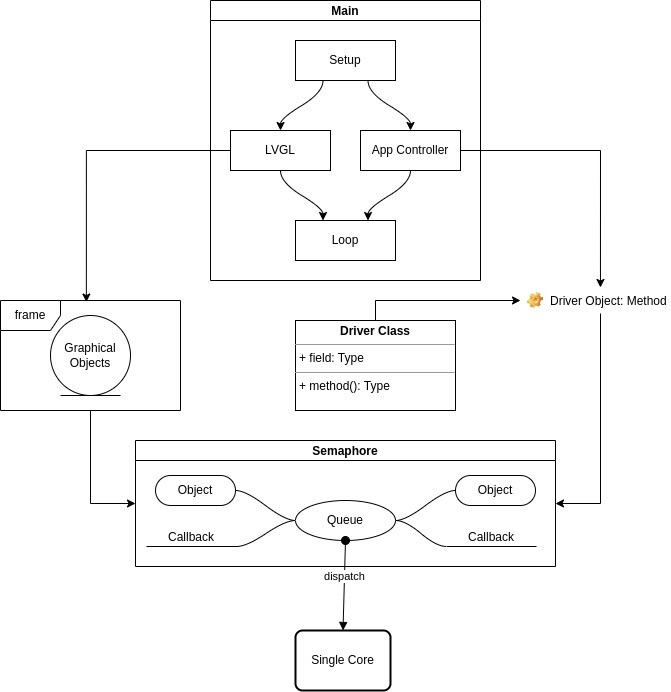
\includegraphics[width=\textwidth]{Figures/firmwareArchitecture.jpg}
        \caption{Firmware architecture}
        \label{fig:firmware_architecture}
    \end{figure}
    The application starts in the main function where time tickers have been created for updating the UI. A low-priority thread was created for handling the GUI, basically updating and refreshing the GUI elements every 200ms. Another above-normal priority thread is also created with an event queue for handling the business logic of the application. This thread is controlled by an app controller class, which takes in the objects, functions, and function arguments of the driver classes and dispatches this into an event queue as events. Once an event has been dispatched, it can be canceled but it is unsafe as might lead to a memory leak. 
    \par 
    The graphical objects have callbacks assigned to only certain events they might generate. Such callbacks communicate with the app controller thread using a semaphore and dispatch an event into the queue. This is handled by the single core on the microcontroller board.

    \item \textbf{Wired Remote Control}\\
    The firmware for this application also supports remote control over an ethernet cable. This is enabled by a W5500 ethernet module onboard the electronics board. This type of control is also enabled by a desktop application shown in figure \ref{fig:desktop_application} made specifically for this application.
    The communication between the PC, and the microcontroller board is through a protobuf protocol with typed fields.
    \par
    The setup for this type of control starts with setting a static IP address in a PC and then connecting the PC to the W5500 ethernet module, onboard the system. The same PC's static IP address is also inserted in the IP text fields on screen 2 of the application.  The port is kept at 1883. The connection is established once the connect button is clicked.
    \begin{figure}[H]
        \centering
        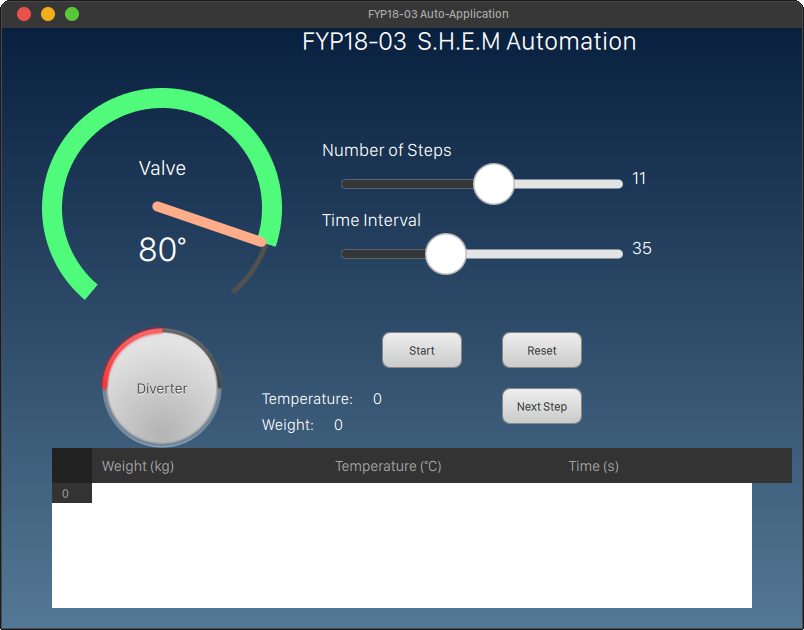
\includegraphics[width=\textwidth]{Figures/desktop_v1.png}
        \caption{Desktop application }
        \label{fig:desktop_application}
    \end{figure}
\end{itemize}